\documentclass[twoside]{book}

% Packages required by doxygen
\usepackage{fixltx2e}
\usepackage{calc}
\usepackage{doxygen}
\usepackage[export]{adjustbox} % also loads graphicx
\usepackage{graphicx}
\usepackage[utf8]{inputenc}
\usepackage{makeidx}
\usepackage{multicol}
\usepackage{multirow}
\PassOptionsToPackage{warn}{textcomp}
\usepackage{textcomp}
\usepackage[nointegrals]{wasysym}
\usepackage[table]{xcolor}

% Font selection
\usepackage[T1]{fontenc}
\usepackage[scaled=.90]{helvet}
\usepackage{courier}
\usepackage{amssymb}
\usepackage{sectsty}
\renewcommand{\familydefault}{\sfdefault}
\allsectionsfont{%
  \fontseries{bc}\selectfont%
  \color{darkgray}%
}
\renewcommand{\DoxyLabelFont}{%
  \fontseries{bc}\selectfont%
  \color{darkgray}%
}
\newcommand{\+}{\discretionary{\mbox{\scriptsize$\hookleftarrow$}}{}{}}

% Page & text layout
\usepackage{geometry}
\geometry{%
  a4paper,%
  top=2.5cm,%
  bottom=2.5cm,%
  left=2.5cm,%
  right=2.5cm%
}
\tolerance=750
\hfuzz=15pt
\hbadness=750
\setlength{\emergencystretch}{15pt}
\setlength{\parindent}{0cm}
\setlength{\parskip}{3ex plus 2ex minus 2ex}
\makeatletter
\renewcommand{\paragraph}{%
  \@startsection{paragraph}{4}{0ex}{-1.0ex}{1.0ex}{%
    \normalfont\normalsize\bfseries\SS@parafont%
  }%
}
\renewcommand{\subparagraph}{%
  \@startsection{subparagraph}{5}{0ex}{-1.0ex}{1.0ex}{%
    \normalfont\normalsize\bfseries\SS@subparafont%
  }%
}
\makeatother

% Headers & footers
\usepackage{fancyhdr}
\pagestyle{fancyplain}
\fancyhead[LE]{\fancyplain{}{\bfseries\thepage}}
\fancyhead[CE]{\fancyplain{}{}}
\fancyhead[RE]{\fancyplain{}{\bfseries\leftmark}}
\fancyhead[LO]{\fancyplain{}{\bfseries\rightmark}}
\fancyhead[CO]{\fancyplain{}{}}
\fancyhead[RO]{\fancyplain{}{\bfseries\thepage}}
\fancyfoot[LE]{\fancyplain{}{}}
\fancyfoot[CE]{\fancyplain{}{}}
\fancyfoot[RE]{\fancyplain{}{\bfseries\scriptsize Generated by Doxygen }}
\fancyfoot[LO]{\fancyplain{}{\bfseries\scriptsize Generated by Doxygen }}
\fancyfoot[CO]{\fancyplain{}{}}
\fancyfoot[RO]{\fancyplain{}{}}
\renewcommand{\footrulewidth}{0.4pt}
\renewcommand{\chaptermark}[1]{%
  \markboth{#1}{}%
}
\renewcommand{\sectionmark}[1]{%
  \markright{\thesection\ #1}%
}

% Indices & bibliography
\usepackage{natbib}
\usepackage[titles]{tocloft}
\setcounter{tocdepth}{3}
\setcounter{secnumdepth}{5}
\makeindex

% Hyperlinks (required, but should be loaded last)
\usepackage{ifpdf}
\ifpdf
  \usepackage[pdftex,pagebackref=true]{hyperref}
\else
  \usepackage[ps2pdf,pagebackref=true]{hyperref}
\fi
\hypersetup{%
  colorlinks=true,%
  linkcolor=blue,%
  citecolor=blue,%
  unicode%
}

% Custom commands
\newcommand{\clearemptydoublepage}{%
  \newpage{\pagestyle{empty}\cleardoublepage}%
}

\usepackage{caption}
\captionsetup{labelsep=space,justification=centering,font={bf},singlelinecheck=off,skip=4pt,position=top}

%===== C O N T E N T S =====

\begin{document}

% Titlepage & ToC
\hypersetup{pageanchor=false,
             bookmarksnumbered=true,
             pdfencoding=unicode
            }
\pagenumbering{alph}
\begin{titlepage}
\vspace*{7cm}
\begin{center}%
{\Large My Project }\\
\vspace*{1cm}
{\large Generated by Doxygen 1.8.13}\\
\end{center}
\end{titlepage}
\clearemptydoublepage
\pagenumbering{roman}
\tableofcontents
\clearemptydoublepage
\pagenumbering{arabic}
\hypersetup{pageanchor=true}

%--- Begin generated contents ---
\chapter{R\+E\+A\+D\+ME}
\label{md_README}
\Hypertarget{md_README}
project source 
\chapter{Class Index}
\section{Class List}
Here are the classes, structs, unions and interfaces with brief descriptions\+:\begin{DoxyCompactList}
\item\contentsline{section}{\hyperlink{structbucket}{bucket} }{\pageref{structbucket}}{}
\item\contentsline{section}{\hyperlink{structbucketf}{bucketf} }{\pageref{structbucketf}}{}
\item\contentsline{section}{\hyperlink{structbucketv}{bucketv} }{\pageref{structbucketv}}{}
\item\contentsline{section}{\hyperlink{structcl}{cl} }{\pageref{structcl}}{}
\item\contentsline{section}{\hyperlink{structfat}{fat} }{\pageref{structfat}}{}
\item\contentsline{section}{\hyperlink{structfil}{fil} }{\pageref{structfil}}{}
\item\contentsline{section}{\hyperlink{structfili}{fili} }{\pageref{structfili}}{}
\item\contentsline{section}{\hyperlink{structfilial}{filial} }{\pageref{structfilial}}{}
\item\contentsline{section}{\hyperlink{structmes}{mes} }{\pageref{structmes}}{}
\item\contentsline{section}{\hyperlink{structmesf}{mesf} }{\pageref{structmesf}}{}
\item\contentsline{section}{\hyperlink{structprd}{prd} }{\pageref{structprd}}{}
\item\contentsline{section}{\hyperlink{structqprd}{qprd} }{\pageref{structqprd}}{}
\item\contentsline{section}{\hyperlink{structsgv}{sgv} }{\pageref{structsgv}}{}
\item\contentsline{section}{\hyperlink{structthash}{thash} }{\pageref{structthash}}{}
\end{DoxyCompactList}

\chapter{File Index}
\section{File List}
Here is a list of all documented files with brief descriptions\+:\begin{DoxyCompactList}
\item\contentsline{section}{\hyperlink{clientes_8c}{clientes.\+c} \\*Modulo que contém as funcções para leitura e validação de clientes }{\pageref{clientes_8c}}{}
\item\contentsline{section}{\hyperlink{faturacao_8c}{faturacao.\+c} \\*Modulo que contém as funcções para processamento, validação de faturas }{\pageref{faturacao_8c}}{}
\item\contentsline{section}{\hyperlink{filiais_8c}{filiais.\+c} \\*Modulo que contém as funcções para a gestão das filiais }{\pageref{filiais_8c}}{}
\item\contentsline{section}{\hyperlink{interface_8c}{interface.\+c} \\*Modulo que contém as funcções para apresentação das respostas as queries }{\pageref{interface_8c}}{}
\item\contentsline{section}{\hyperlink{main_8c}{main.\+c} \\*Modulo main }{\pageref{main_8c}}{}
\item\contentsline{section}{\hyperlink{produtos_8c}{produtos.\+c} \\*Modulo que contém as funções para leitura e validação de produtos }{\pageref{produtos_8c}}{}
\item\contentsline{section}{\hyperlink{queries_8c}{queries.\+c} \\*Modulo que contém as funcções de resposta as queries }{\pageref{queries_8c}}{}
\item\contentsline{section}{\hyperlink{vendas_8c}{vendas.\+c} \\*Modulo que contém as funcções para leitura e validação de vendas e incorporação destas nas estruturas filiais e faturação }{\pageref{vendas_8c}}{}
\end{DoxyCompactList}

\chapter{Class Documentation}
\hypertarget{structbucket}{}\section{bucket Struct Reference}
\label{structbucket}\index{bucket@{bucket}}
\subsection*{Public Attributes}
\begin{DoxyCompactItemize}
\item 
\mbox{\Hypertarget{structbucket_afe82634d6f8552dffc3097139434a407}\label{structbucket_afe82634d6f8552dffc3097139434a407}} 
int {\bfseries size}
\item 
\mbox{\Hypertarget{structbucket_ad7541adf4a0ecad66f5c5f34581dedaf}\label{structbucket_ad7541adf4a0ecad66f5c5f34581dedaf}} 
char $\ast$$\ast$ {\bfseries arr}
\end{DoxyCompactItemize}


The documentation for this struct was generated from the following files\+:\begin{DoxyCompactItemize}
\item 
\hyperlink{clientes_8c}{clientes.\+c}\item 
\hyperlink{produtos_8c}{produtos.\+c}\end{DoxyCompactItemize}

\hypertarget{structbucketf}{}\section{bucketf Struct Reference}
\label{structbucketf}\index{bucketf@{bucketf}}


Collaboration diagram for bucketf\+:
\nopagebreak
\begin{figure}[H]
\begin{center}
\leavevmode
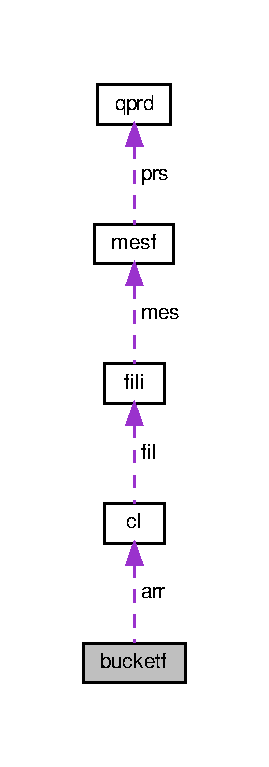
\includegraphics[width=129pt]{structbucketf__coll__graph}
\end{center}
\end{figure}
\subsection*{Public Attributes}
\begin{DoxyCompactItemize}
\item 
\mbox{\Hypertarget{structbucketf_acadddf33dfda3ab216eab6537cb79691}\label{structbucketf_acadddf33dfda3ab216eab6537cb79691}} 
int {\bfseries size}
\item 
\mbox{\Hypertarget{structbucketf_ab98d2c8f780f43c782a92b9d6836e1cb}\label{structbucketf_ab98d2c8f780f43c782a92b9d6836e1cb}} 
\hyperlink{structcl}{Cl} $\ast$ {\bfseries arr}
\end{DoxyCompactItemize}


The documentation for this struct was generated from the following file\+:\begin{DoxyCompactItemize}
\item 
\hyperlink{filiais_8c}{filiais.\+c}\end{DoxyCompactItemize}

\hypertarget{structbucketv}{}\section{bucketv Struct Reference}
\label{structbucketv}\index{bucketv@{bucketv}}


Collaboration diagram for bucketv\+:
\nopagebreak
\begin{figure}[H]
\begin{center}
\leavevmode
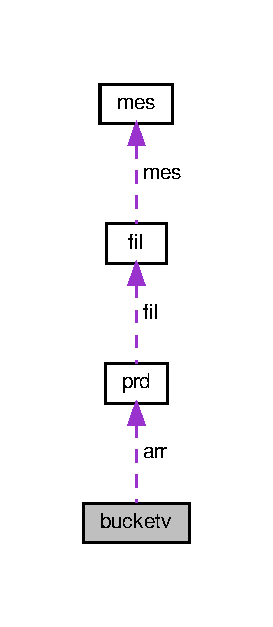
\includegraphics[width=131pt]{structbucketv__coll__graph}
\end{center}
\end{figure}
\subsection*{Public Attributes}
\begin{DoxyCompactItemize}
\item 
\mbox{\Hypertarget{structbucketv_ad6d992292eafe2b9e38ae633e07a2f7b}\label{structbucketv_ad6d992292eafe2b9e38ae633e07a2f7b}} 
int {\bfseries size}
\item 
\mbox{\Hypertarget{structbucketv_a8890f3fe25c884f2acd544722f31a987}\label{structbucketv_a8890f3fe25c884f2acd544722f31a987}} 
\hyperlink{structprd}{Prd} $\ast$ {\bfseries arr}
\end{DoxyCompactItemize}


The documentation for this struct was generated from the following file\+:\begin{DoxyCompactItemize}
\item 
\hyperlink{faturacao_8c}{faturacao.\+c}\end{DoxyCompactItemize}

\hypertarget{structcl}{}\section{cl Struct Reference}
\label{structcl}\index{cl@{cl}}


Collaboration diagram for cl\+:
\nopagebreak
\begin{figure}[H]
\begin{center}
\leavevmode
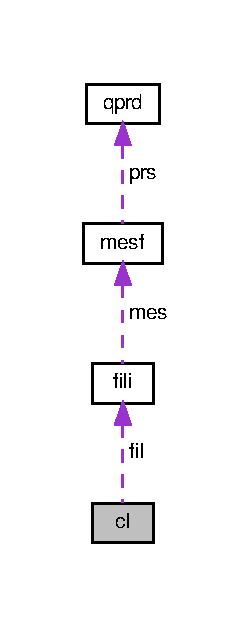
\includegraphics[width=121pt]{structcl__coll__graph}
\end{center}
\end{figure}
\subsection*{Public Attributes}
\begin{DoxyCompactItemize}
\item 
\mbox{\Hypertarget{structcl_a0387de3ebf25a3eca5713185b874d576}\label{structcl_a0387de3ebf25a3eca5713185b874d576}} 
char $\ast$ {\bfseries cid}
\item 
\mbox{\Hypertarget{structcl_a01e86c9d03698621304fceb71c47866c}\label{structcl_a01e86c9d03698621304fceb71c47866c}} 
\hyperlink{structfili}{Fili} $\ast$ {\bfseries fil}
\end{DoxyCompactItemize}


The documentation for this struct was generated from the following file\+:\begin{DoxyCompactItemize}
\item 
\hyperlink{filiais_8c}{filiais.\+c}\end{DoxyCompactItemize}

\hypertarget{structfat}{}\section{fat Struct Reference}
\label{structfat}\index{fat@{fat}}


Collaboration diagram for fat\+:
\nopagebreak
\begin{figure}[H]
\begin{center}
\leavevmode
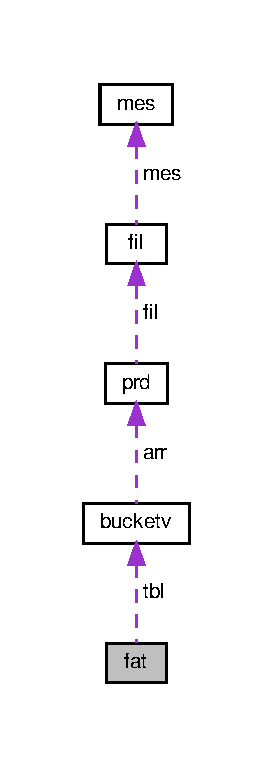
\includegraphics[width=131pt]{structfat__coll__graph}
\end{center}
\end{figure}
\subsection*{Public Attributes}
\begin{DoxyCompactItemize}
\item 
\mbox{\Hypertarget{structfat_a2e88d3f6590a682cd4fd5bac64172eed}\label{structfat_a2e88d3f6590a682cd4fd5bac64172eed}} 
\hyperlink{structbucketv}{Bucketv} $\ast$ {\bfseries tbl}
\end{DoxyCompactItemize}


The documentation for this struct was generated from the following file\+:\begin{DoxyCompactItemize}
\item 
\hyperlink{faturacao_8c}{faturacao.\+c}\end{DoxyCompactItemize}

\hypertarget{structfil}{}\section{fil Struct Reference}
\label{structfil}\index{fil@{fil}}


Collaboration diagram for fil\+:
\nopagebreak
\begin{figure}[H]
\begin{center}
\leavevmode
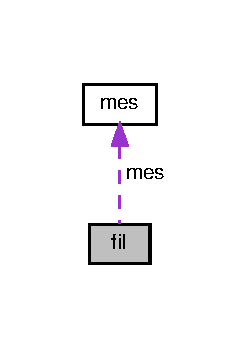
\includegraphics[width=120pt]{structfil__coll__graph}
\end{center}
\end{figure}
\subsection*{Public Attributes}
\begin{DoxyCompactItemize}
\item 
\mbox{\Hypertarget{structfil_a33ff794e38a053923179cf7bc1b1ac48}\label{structfil_a33ff794e38a053923179cf7bc1b1ac48}} 
int {\bfseries used}
\item 
\mbox{\Hypertarget{structfil_a6837e994f9fa4c7c9db93dff06600b8b}\label{structfil_a6837e994f9fa4c7c9db93dff06600b8b}} 
\hyperlink{structmes}{Mes} $\ast$ {\bfseries mes}
\end{DoxyCompactItemize}


The documentation for this struct was generated from the following file\+:\begin{DoxyCompactItemize}
\item 
\hyperlink{faturacao_8c}{faturacao.\+c}\end{DoxyCompactItemize}

\hypertarget{structfili}{}\section{fili Struct Reference}
\label{structfili}\index{fili@{fili}}


Collaboration diagram for fili\+:
\nopagebreak
\begin{figure}[H]
\begin{center}
\leavevmode
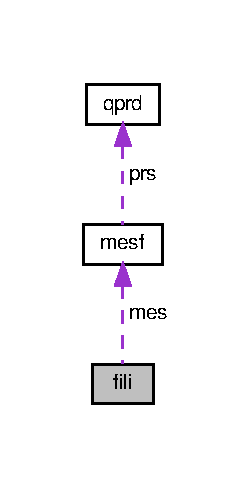
\includegraphics[width=121pt]{structfili__coll__graph}
\end{center}
\end{figure}
\subsection*{Public Attributes}
\begin{DoxyCompactItemize}
\item 
\mbox{\Hypertarget{structfili_a230d92e837158bb685ac8c5093e96bfd}\label{structfili_a230d92e837158bb685ac8c5093e96bfd}} 
int {\bfseries used}
\item 
\mbox{\Hypertarget{structfili_a928e63db2f379f26cf27fa73e02c3c3d}\label{structfili_a928e63db2f379f26cf27fa73e02c3c3d}} 
\hyperlink{structmesf}{Mesf} $\ast$ {\bfseries mes}
\end{DoxyCompactItemize}


The documentation for this struct was generated from the following file\+:\begin{DoxyCompactItemize}
\item 
\hyperlink{filiais_8c}{filiais.\+c}\end{DoxyCompactItemize}

\hypertarget{structfilial}{}\section{filial Struct Reference}
\label{structfilial}\index{filial@{filial}}


Collaboration diagram for filial\+:
\nopagebreak
\begin{figure}[H]
\begin{center}
\leavevmode
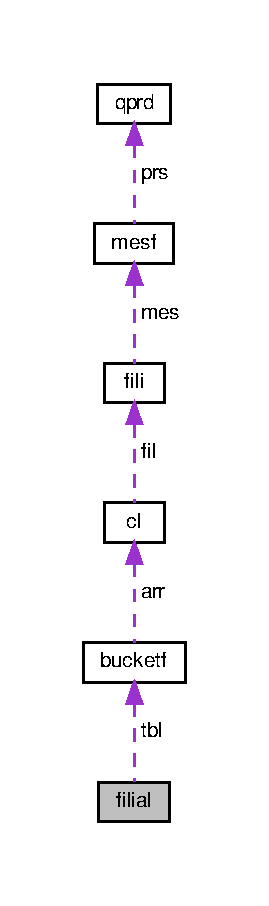
\includegraphics[width=129pt]{structfilial__coll__graph}
\end{center}
\end{figure}
\subsection*{Public Attributes}
\begin{DoxyCompactItemize}
\item 
\mbox{\Hypertarget{structfilial_a5359322cd99e7c14e9af0f7e0d16daf8}\label{structfilial_a5359322cd99e7c14e9af0f7e0d16daf8}} 
\hyperlink{structbucketf}{Bucketf} $\ast$ {\bfseries tbl}
\end{DoxyCompactItemize}


The documentation for this struct was generated from the following file\+:\begin{DoxyCompactItemize}
\item 
\hyperlink{filiais_8c}{filiais.\+c}\end{DoxyCompactItemize}

\hypertarget{structmes}{}\section{mes Struct Reference}
\label{structmes}\index{mes@{mes}}
\subsection*{Public Attributes}
\begin{DoxyCompactItemize}
\item 
\mbox{\Hypertarget{structmes_a233faa087acc8274fc2fcd060537c50f}\label{structmes_a233faa087acc8274fc2fcd060537c50f}} 
double {\bfseries fN}
\item 
\mbox{\Hypertarget{structmes_a1dd8217f43e6fafe71da4535dc5c824c}\label{structmes_a1dd8217f43e6fafe71da4535dc5c824c}} 
double {\bfseries fP}
\item 
\mbox{\Hypertarget{structmes_a65f04ca66c4b34316e8ba88271ec2884}\label{structmes_a65f04ca66c4b34316e8ba88271ec2884}} 
int {\bfseries vN}
\item 
\mbox{\Hypertarget{structmes_a42ca395167be0938b11b7712804418d5}\label{structmes_a42ca395167be0938b11b7712804418d5}} 
int {\bfseries vP}
\end{DoxyCompactItemize}


The documentation for this struct was generated from the following file\+:\begin{DoxyCompactItemize}
\item 
\hyperlink{faturacao_8c}{faturacao.\+c}\end{DoxyCompactItemize}

\hypertarget{structmesf}{}\section{mesf Struct Reference}
\label{structmesf}\index{mesf@{mesf}}


Collaboration diagram for mesf\+:
\nopagebreak
\begin{figure}[H]
\begin{center}
\leavevmode
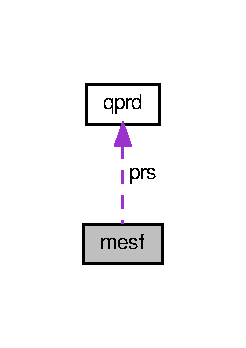
\includegraphics[width=118pt]{structmesf__coll__graph}
\end{center}
\end{figure}
\subsection*{Public Attributes}
\begin{DoxyCompactItemize}
\item 
\mbox{\Hypertarget{structmesf_a719adfb67149cf6a5f2336d4f9c32099}\label{structmesf_a719adfb67149cf6a5f2336d4f9c32099}} 
int {\bfseries size}
\item 
\mbox{\Hypertarget{structmesf_a67f98166aa2c830b4ca93ff63751a8c3}\label{structmesf_a67f98166aa2c830b4ca93ff63751a8c3}} 
\hyperlink{structqprd}{Qprd} $\ast$ {\bfseries prs}
\end{DoxyCompactItemize}


The documentation for this struct was generated from the following file\+:\begin{DoxyCompactItemize}
\item 
\hyperlink{filiais_8c}{filiais.\+c}\end{DoxyCompactItemize}

\hypertarget{structprd}{}\section{prd Struct Reference}
\label{structprd}\index{prd@{prd}}


Collaboration diagram for prd\+:
\nopagebreak
\begin{figure}[H]
\begin{center}
\leavevmode
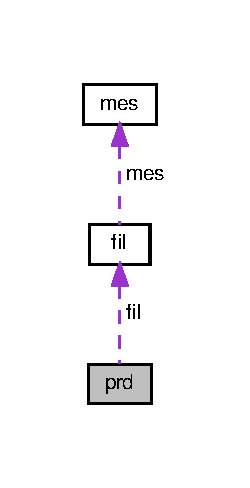
\includegraphics[width=120pt]{structprd__coll__graph}
\end{center}
\end{figure}
\subsection*{Public Attributes}
\begin{DoxyCompactItemize}
\item 
\mbox{\Hypertarget{structprd_ab263af87d7d5939e74048142eef82bba}\label{structprd_ab263af87d7d5939e74048142eef82bba}} 
char $\ast$ {\bfseries pid}
\item 
\mbox{\Hypertarget{structprd_a0f71e040e3697d8283952ae3a0cd7f81}\label{structprd_a0f71e040e3697d8283952ae3a0cd7f81}} 
\hyperlink{structfil}{Fil} $\ast$ {\bfseries fil}
\end{DoxyCompactItemize}


The documentation for this struct was generated from the following file\+:\begin{DoxyCompactItemize}
\item 
\hyperlink{faturacao_8c}{faturacao.\+c}\end{DoxyCompactItemize}

\hypertarget{structqprd}{}\section{qprd Struct Reference}
\label{structqprd}\index{qprd@{qprd}}
\subsection*{Public Attributes}
\begin{DoxyCompactItemize}
\item 
\mbox{\Hypertarget{structqprd_abedcf4ae333edcd9459c465ae54e1516}\label{structqprd_abedcf4ae333edcd9459c465ae54e1516}} 
char $\ast$ {\bfseries pid}
\item 
\mbox{\Hypertarget{structqprd_a319485158a8384134df4c7b9c4765296}\label{structqprd_a319485158a8384134df4c7b9c4765296}} 
int {\bfseries qN}
\item 
\mbox{\Hypertarget{structqprd_a87236da95deac1b42e3ac9b3d42d8f57}\label{structqprd_a87236da95deac1b42e3ac9b3d42d8f57}} 
int {\bfseries qP}
\item 
\mbox{\Hypertarget{structqprd_a437795ceda0ff87bb01579c64d44b7a7}\label{structqprd_a437795ceda0ff87bb01579c64d44b7a7}} 
double {\bfseries gN}
\item 
\mbox{\Hypertarget{structqprd_a75c8fcf02e25e6b2f15c0d17645c1881}\label{structqprd_a75c8fcf02e25e6b2f15c0d17645c1881}} 
double {\bfseries gP}
\end{DoxyCompactItemize}


The documentation for this struct was generated from the following file\+:\begin{DoxyCompactItemize}
\item 
\hyperlink{filiais_8c}{filiais.\+c}\end{DoxyCompactItemize}

\hypertarget{structsgv}{}\section{sgv Struct Reference}
\label{structsgv}\index{sgv@{sgv}}


Collaboration diagram for sgv\+:
\nopagebreak
\begin{figure}[H]
\begin{center}
\leavevmode
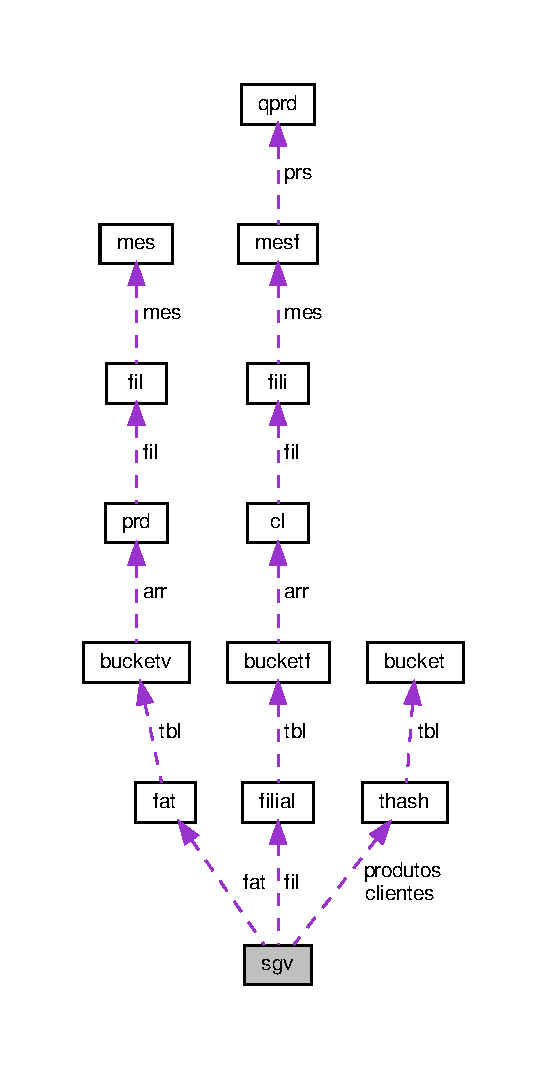
\includegraphics[width=263pt]{structsgv__coll__graph}
\end{center}
\end{figure}
\subsection*{Public Attributes}
\begin{DoxyCompactItemize}
\item 
\mbox{\Hypertarget{structsgv_a4b8d7e6a972ec2f21671b3ab155d132a}\label{structsgv_a4b8d7e6a972ec2f21671b3ab155d132a}} 
int {\bfseries pv}
\item 
\mbox{\Hypertarget{structsgv_a36bc956c45e586a9b9056deeb1749a6b}\label{structsgv_a36bc956c45e586a9b9056deeb1749a6b}} 
int {\bfseries cv}
\item 
\mbox{\Hypertarget{structsgv_a2d080a4c47b473d8747e89c18735d8f3}\label{structsgv_a2d080a4c47b473d8747e89c18735d8f3}} 
int {\bfseries vv}
\item 
\mbox{\Hypertarget{structsgv_a02e1e045823a4dc3c1ab1ece027a5b4a}\label{structsgv_a02e1e045823a4dc3c1ab1ece027a5b4a}} 
int {\bfseries pl}
\item 
\mbox{\Hypertarget{structsgv_adac44502afdca954fd3b57b829e2b049}\label{structsgv_adac44502afdca954fd3b57b829e2b049}} 
int {\bfseries cl}
\item 
\mbox{\Hypertarget{structsgv_ad95470ebda9ad32f6dbecaa30ea14cd5}\label{structsgv_ad95470ebda9ad32f6dbecaa30ea14cd5}} 
int {\bfseries vl}
\item 
\mbox{\Hypertarget{structsgv_a317521860330be926e28125e899c58ea}\label{structsgv_a317521860330be926e28125e899c58ea}} 
char $\ast$ {\bfseries p}
\item 
\mbox{\Hypertarget{structsgv_a82cc554aef081b2f7503dc5566fbf04e}\label{structsgv_a82cc554aef081b2f7503dc5566fbf04e}} 
char $\ast$ {\bfseries c}
\item 
\mbox{\Hypertarget{structsgv_afe9a282ca6b9d987c53776d4e929e947}\label{structsgv_afe9a282ca6b9d987c53776d4e929e947}} 
char $\ast$ {\bfseries v}
\item 
\mbox{\Hypertarget{structsgv_a47f0cef78e0698ee4ece6c6258bb34d8}\label{structsgv_a47f0cef78e0698ee4ece6c6258bb34d8}} 
\hyperlink{structthash}{T\+Hash} $\ast$ {\bfseries produtos}
\item 
\mbox{\Hypertarget{structsgv_af18caa4720ba06601ff5e040ed8617a3}\label{structsgv_af18caa4720ba06601ff5e040ed8617a3}} 
\hyperlink{structthash}{T\+Hash} $\ast$ {\bfseries clientes}
\item 
\mbox{\Hypertarget{structsgv_a33a097883450d211c75b3c2c98b658eb}\label{structsgv_a33a097883450d211c75b3c2c98b658eb}} 
\hyperlink{structfat}{Fat} $\ast$ {\bfseries fat}
\item 
\mbox{\Hypertarget{structsgv_aa600935a1125d376845c0368238bf0b1}\label{structsgv_aa600935a1125d376845c0368238bf0b1}} 
\hyperlink{structfilial}{Filial} $\ast$ {\bfseries fil}
\end{DoxyCompactItemize}


The documentation for this struct was generated from the following file\+:\begin{DoxyCompactItemize}
\item 
\hyperlink{queries_8c}{queries.\+c}\end{DoxyCompactItemize}

\hypertarget{structthash}{}\section{thash Struct Reference}
\label{structthash}\index{thash@{thash}}


Collaboration diagram for thash\+:
\nopagebreak
\begin{figure}[H]
\begin{center}
\leavevmode
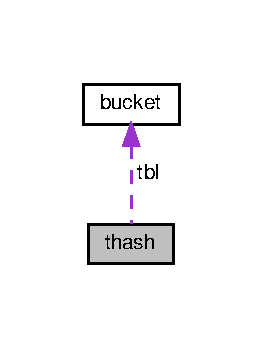
\includegraphics[width=126pt]{structthash__coll__graph}
\end{center}
\end{figure}
\subsection*{Public Attributes}
\begin{DoxyCompactItemize}
\item 
\mbox{\Hypertarget{structthash_a1ab8265f26cdd44c63cc812b0b56dab5}\label{structthash_a1ab8265f26cdd44c63cc812b0b56dab5}} 
int {\bfseries size}
\item 
\mbox{\Hypertarget{structthash_aaf099d908ffbfc2d8ad138e2a3af94e8}\label{structthash_aaf099d908ffbfc2d8ad138e2a3af94e8}} 
\hyperlink{structbucket}{Bucket} $\ast$ {\bfseries tbl}
\end{DoxyCompactItemize}


The documentation for this struct was generated from the following files\+:\begin{DoxyCompactItemize}
\item 
\hyperlink{clientes_8c}{clientes.\+c}\item 
\hyperlink{produtos_8c}{produtos.\+c}\end{DoxyCompactItemize}

\chapter{File Documentation}
\hypertarget{clientes_8c}{}\section{clientes.\+c File Reference}
\label{clientes_8c}\index{clientes.\+c@{clientes.\+c}}


Modulo que contém as funcções para leitura e validação de clientes.  


{\ttfamily \#include $<$stdio.\+h$>$}\newline
{\ttfamily \#include $<$string.\+h$>$}\newline
{\ttfamily \#include $<$stdlib.\+h$>$}\newline
{\ttfamily \#include \char`\"{}clientes.\+h\char`\"{}}\newline
Include dependency graph for clientes.\+c\+:
\nopagebreak
\begin{figure}[H]
\begin{center}
\leavevmode
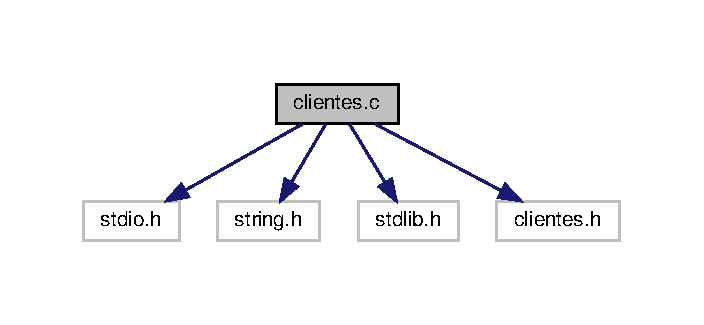
\includegraphics[width=338pt]{clientes_8c__incl}
\end{center}
\end{figure}
\subsection*{Classes}
\begin{DoxyCompactItemize}
\item 
struct \hyperlink{structbucket}{bucket}
\item 
struct \hyperlink{structthash}{thash}
\end{DoxyCompactItemize}
\subsection*{Typedefs}
\begin{DoxyCompactItemize}
\item 
\mbox{\Hypertarget{clientes_8c_ab73320ba1511b228e2d4df6fa47e8f1d}\label{clientes_8c_ab73320ba1511b228e2d4df6fa47e8f1d}} 
typedef struct \hyperlink{structbucket}{bucket} {\bfseries Bucket}
\item 
\mbox{\Hypertarget{clientes_8c_a21f0028bc00faa3267e3e3cc9ff2e271}\label{clientes_8c_a21f0028bc00faa3267e3e3cc9ff2e271}} 
typedef struct \hyperlink{structthash}{thash} {\bfseries T\+Hash}
\end{DoxyCompactItemize}
\subsection*{Functions}
\begin{DoxyCompactItemize}
\item 
int \hyperlink{clientes_8c_af88c9cf612c7bfaca1afd182d302306a}{hash} (char $\ast$cont)
\begin{DoxyCompactList}\small\item\em Função que recebe uma string e subtrai ao primeiro elemnto da string a letra A. \end{DoxyCompactList}\item 
\hyperlink{structthash}{T\+Hash} $\ast$ \hyperlink{clientes_8c_abdf1fc124ed891a05dba7d1fce51dfcc}{init\+Tab} ()
\begin{DoxyCompactList}\small\item\em Função que inicia uma estrutura Thash alocando espaço para todas as estruturas adjacentes. \end{DoxyCompactList}\item 
void \hyperlink{clientes_8c_a02a7235067818588fbfbe3121e42b34d}{destroi\+Tab} (\hyperlink{structthash}{T\+Hash} $\ast$h)
\begin{DoxyCompactList}\small\item\em Funçao que destroi uma estrutura Thash libertando o espaço ocupado por esta. \end{DoxyCompactList}\item 
void \hyperlink{clientes_8c_a88acb4c6adff7ed545eaa56c3c8d9d5b}{acrecensta\+Tab} (\hyperlink{structthash}{T\+Hash} $\ast$h, char $\ast$cont)
\begin{DoxyCompactList}\small\item\em Função que acrescenta a uma Thash uma derminada string. \end{DoxyCompactList}\item 
void \hyperlink{clientes_8c_a0e8f326da95dbd031e75a42e98b2a45d}{swapc} (char $\ast$$\ast$arg1, char $\ast$$\ast$arg2)
\begin{DoxyCompactList}\small\item\em Função que troca duas strings de posicao. \end{DoxyCompactList}\item 
void \hyperlink{clientes_8c_ae91c7810753de46884a5784decc2e710}{quicksortc} (char $\ast$$\ast$args, unsigned int len)
\begin{DoxyCompactList}\small\item\em Função que ordena um array de strings. \end{DoxyCompactList}\item 
int \hyperlink{clientes_8c_aea63038230f76b0df401d2740dace813}{ler\+\_\+clientes} (\hyperlink{structthash}{T\+Hash} $\ast$cliente, char $\ast$filespath, int $\ast$c)
\begin{DoxyCompactList}\small\item\em Função que le de um ficheiro para uma Thash. \end{DoxyCompactList}\item 
int \hyperlink{clientes_8c_a50ddba9ef7134b08d60d7e478e73d475}{validacliente} (char $\ast$cliente)
\begin{DoxyCompactList}\small\item\em Função que recebe uma string de um cliente e verifica se este é valido. \end{DoxyCompactList}\item 
char $\ast$ \hyperlink{clientes_8c_abbac116a2a21355d9e177a2fc9a909d3}{get\+Cliente} (\hyperlink{structthash}{T\+Hash} $\ast$c, int key, int i)
\begin{DoxyCompactList}\small\item\em Função que cria um clone de uma string cliente. \end{DoxyCompactList}\item 
char $\ast$$\ast$ \hyperlink{clientes_8c_a638742b0dbf906ab1adddae05a59a0d7}{get\+Array\+Cl} (\hyperlink{structthash}{T\+Hash} $\ast$c, int key)
\begin{DoxyCompactList}\small\item\em Função que cria um clone de um array de strings cliente. \end{DoxyCompactList}\item 
int \hyperlink{clientes_8c_a65b82751aa341222148fbe9a6e6603cd}{get\+Array\+Cl\+Size} (\hyperlink{structthash}{T\+Hash} $\ast$c, int key)
\begin{DoxyCompactList}\small\item\em Função que retorna o size um determinado array na tabela. \end{DoxyCompactList}\end{DoxyCompactItemize}


\subsection{Detailed Description}
Modulo que contém as funcções para leitura e validação de clientes. 



\subsection{Function Documentation}
\mbox{\Hypertarget{clientes_8c_a88acb4c6adff7ed545eaa56c3c8d9d5b}\label{clientes_8c_a88acb4c6adff7ed545eaa56c3c8d9d5b}} 
\index{clientes.\+c@{clientes.\+c}!acrecensta\+Tab@{acrecensta\+Tab}}
\index{acrecensta\+Tab@{acrecensta\+Tab}!clientes.\+c@{clientes.\+c}}
\subsubsection{\texorpdfstring{acrecensta\+Tab()}{acrecenstaTab()}}
{\footnotesize\ttfamily void acrecensta\+Tab (\begin{DoxyParamCaption}\item[{\hyperlink{structthash}{T\+Hash} $\ast$}]{h,  }\item[{char $\ast$}]{cont }\end{DoxyParamCaption})}



Função que acrescenta a uma Thash uma derminada string. 

Aplicando a função hash descobre a posicao correta desta na T\+Hash e sucessivamente realocando espaço para a adicionar á mesma


\begin{DoxyParams}{Parameters}
{\em T\+Hash} & $\ast$h T\+Hash previamente inicializada \\
\hline
{\em char} & $\ast$cont String genérica \\
\hline
\end{DoxyParams}
\mbox{\Hypertarget{clientes_8c_a02a7235067818588fbfbe3121e42b34d}\label{clientes_8c_a02a7235067818588fbfbe3121e42b34d}} 
\index{clientes.\+c@{clientes.\+c}!destroi\+Tab@{destroi\+Tab}}
\index{destroi\+Tab@{destroi\+Tab}!clientes.\+c@{clientes.\+c}}
\subsubsection{\texorpdfstring{destroi\+Tab()}{destroiTab()}}
{\footnotesize\ttfamily void destroi\+Tab (\begin{DoxyParamCaption}\item[{\hyperlink{structthash}{T\+Hash} $\ast$}]{h }\end{DoxyParamCaption})}



Funçao que destroi uma estrutura Thash libertando o espaço ocupado por esta. 


\begin{DoxyParams}{Parameters}
{\em T\+Hash} & $\ast$h T\+Hash previamente inicializada \\
\hline
\end{DoxyParams}
\mbox{\Hypertarget{clientes_8c_a638742b0dbf906ab1adddae05a59a0d7}\label{clientes_8c_a638742b0dbf906ab1adddae05a59a0d7}} 
\index{clientes.\+c@{clientes.\+c}!get\+Array\+Cl@{get\+Array\+Cl}}
\index{get\+Array\+Cl@{get\+Array\+Cl}!clientes.\+c@{clientes.\+c}}
\subsubsection{\texorpdfstring{get\+Array\+Cl()}{getArrayCl()}}
{\footnotesize\ttfamily char$\ast$$\ast$ get\+Array\+Cl (\begin{DoxyParamCaption}\item[{\hyperlink{structthash}{T\+Hash} $\ast$}]{c,  }\item[{int}]{key }\end{DoxyParamCaption})}



Função que cria um clone de um array de strings cliente. 


\begin{DoxyParams}{Parameters}
{\em T\+Hash} & $\ast$c Tabela de onde é retirado o cliente \\
\hline
{\em int} & key indice na tabela\\
\hline
\end{DoxyParams}
\begin{DoxyReturn}{Returns}
char$\ast$$\ast$ Retorno da copia 
\end{DoxyReturn}
\mbox{\Hypertarget{clientes_8c_a65b82751aa341222148fbe9a6e6603cd}\label{clientes_8c_a65b82751aa341222148fbe9a6e6603cd}} 
\index{clientes.\+c@{clientes.\+c}!get\+Array\+Cl\+Size@{get\+Array\+Cl\+Size}}
\index{get\+Array\+Cl\+Size@{get\+Array\+Cl\+Size}!clientes.\+c@{clientes.\+c}}
\subsubsection{\texorpdfstring{get\+Array\+Cl\+Size()}{getArrayClSize()}}
{\footnotesize\ttfamily int get\+Array\+Cl\+Size (\begin{DoxyParamCaption}\item[{\hyperlink{structthash}{T\+Hash} $\ast$}]{c,  }\item[{int}]{key }\end{DoxyParamCaption})}



Função que retorna o size um determinado array na tabela. 


\begin{DoxyParams}{Parameters}
{\em T\+Hash} & $\ast$c Tabela de onde é retirado o cliente \\
\hline
{\em int} & key indice na tabela\\
\hline
\end{DoxyParams}
\begin{DoxyReturn}{Returns}
int Retorno do size 
\end{DoxyReturn}
\mbox{\Hypertarget{clientes_8c_abbac116a2a21355d9e177a2fc9a909d3}\label{clientes_8c_abbac116a2a21355d9e177a2fc9a909d3}} 
\index{clientes.\+c@{clientes.\+c}!get\+Cliente@{get\+Cliente}}
\index{get\+Cliente@{get\+Cliente}!clientes.\+c@{clientes.\+c}}
\subsubsection{\texorpdfstring{get\+Cliente()}{getCliente()}}
{\footnotesize\ttfamily char$\ast$ get\+Cliente (\begin{DoxyParamCaption}\item[{\hyperlink{structthash}{T\+Hash} $\ast$}]{c,  }\item[{int}]{key,  }\item[{int}]{i }\end{DoxyParamCaption})}



Função que cria um clone de uma string cliente. 


\begin{DoxyParams}{Parameters}
{\em T\+Hash} & $\ast$c Tabela de onde é retirado o cliente \\
\hline
{\em int} & key indice na tabela \\
\hline
{\em int} & i indice no array\\
\hline
\end{DoxyParams}
\begin{DoxyReturn}{Returns}
char$\ast$ Retorno da copia 
\end{DoxyReturn}
\mbox{\Hypertarget{clientes_8c_af88c9cf612c7bfaca1afd182d302306a}\label{clientes_8c_af88c9cf612c7bfaca1afd182d302306a}} 
\index{clientes.\+c@{clientes.\+c}!hash@{hash}}
\index{hash@{hash}!clientes.\+c@{clientes.\+c}}
\subsubsection{\texorpdfstring{hash()}{hash()}}
{\footnotesize\ttfamily int hash (\begin{DoxyParamCaption}\item[{char $\ast$}]{cont }\end{DoxyParamCaption})}



Função que recebe uma string e subtrai ao primeiro elemnto da string a letra A. 


\begin{DoxyParams}{Parameters}
{\em char} & $\ast$cont String genérica\\
\hline
\end{DoxyParams}
\begin{DoxyReturn}{Returns}
int O resultado inteiro dessa subtração 
\end{DoxyReturn}
\mbox{\Hypertarget{clientes_8c_abdf1fc124ed891a05dba7d1fce51dfcc}\label{clientes_8c_abdf1fc124ed891a05dba7d1fce51dfcc}} 
\index{clientes.\+c@{clientes.\+c}!init\+Tab@{init\+Tab}}
\index{init\+Tab@{init\+Tab}!clientes.\+c@{clientes.\+c}}
\subsubsection{\texorpdfstring{init\+Tab()}{initTab()}}
{\footnotesize\ttfamily \hyperlink{structthash}{T\+Hash}$\ast$ init\+Tab (\begin{DoxyParamCaption}{ }\end{DoxyParamCaption})}



Função que inicia uma estrutura Thash alocando espaço para todas as estruturas adjacentes. 

\begin{DoxyReturn}{Returns}
T\+Hash$\ast$ Devolve a T\+Hash inicializada 
\end{DoxyReturn}
\mbox{\Hypertarget{clientes_8c_aea63038230f76b0df401d2740dace813}\label{clientes_8c_aea63038230f76b0df401d2740dace813}} 
\index{clientes.\+c@{clientes.\+c}!ler\+\_\+clientes@{ler\+\_\+clientes}}
\index{ler\+\_\+clientes@{ler\+\_\+clientes}!clientes.\+c@{clientes.\+c}}
\subsubsection{\texorpdfstring{ler\+\_\+clientes()}{ler\_clientes()}}
{\footnotesize\ttfamily int ler\+\_\+clientes (\begin{DoxyParamCaption}\item[{\hyperlink{structthash}{T\+Hash} $\ast$}]{cliente,  }\item[{char $\ast$}]{filespath,  }\item[{int $\ast$}]{c }\end{DoxyParamCaption})}



Função que le de um ficheiro para uma Thash. 

Recebendo uma Thash e um file path, lê de um ficheiro linha a linha e vai colocando cada linha na thash na sua posição correspondente na mesma


\begin{DoxyParams}{Parameters}
{\em T\+Hash} & $\ast$cliente T\+Hash onde vai ser colocada a informação \\
\hline
{\em char} & $\ast$filespath String com o file path \\
\hline
{\em int} & $\ast$c Inteiro onde é guardado o numero de clientes lidos\\
\hline
\end{DoxyParams}
\begin{DoxyReturn}{Returns}
int O numero de clientes válidos 
\end{DoxyReturn}
\mbox{\Hypertarget{clientes_8c_ae91c7810753de46884a5784decc2e710}\label{clientes_8c_ae91c7810753de46884a5784decc2e710}} 
\index{clientes.\+c@{clientes.\+c}!quicksortc@{quicksortc}}
\index{quicksortc@{quicksortc}!clientes.\+c@{clientes.\+c}}
\subsubsection{\texorpdfstring{quicksortc()}{quicksortc()}}
{\footnotesize\ttfamily void quicksortc (\begin{DoxyParamCaption}\item[{char $\ast$$\ast$}]{args,  }\item[{unsigned int}]{len }\end{DoxyParamCaption})}



Função que ordena um array de strings. 


\begin{DoxyParams}{Parameters}
{\em unsigned} & int len int tam generico \\
\hline
{\em char} & $\ast$$\ast$args String genérica \\
\hline
\end{DoxyParams}
\mbox{\Hypertarget{clientes_8c_a0e8f326da95dbd031e75a42e98b2a45d}\label{clientes_8c_a0e8f326da95dbd031e75a42e98b2a45d}} 
\index{clientes.\+c@{clientes.\+c}!swapc@{swapc}}
\index{swapc@{swapc}!clientes.\+c@{clientes.\+c}}
\subsubsection{\texorpdfstring{swapc()}{swapc()}}
{\footnotesize\ttfamily void swapc (\begin{DoxyParamCaption}\item[{char $\ast$$\ast$}]{arg1,  }\item[{char $\ast$$\ast$}]{arg2 }\end{DoxyParamCaption})}



Função que troca duas strings de posicao. 


\begin{DoxyParams}{Parameters}
{\em char} & $\ast$$\ast$arg1 String genérica \\
\hline
{\em char} & $\ast$$\ast$arg2 String genérica \\
\hline
\end{DoxyParams}
\mbox{\Hypertarget{clientes_8c_a50ddba9ef7134b08d60d7e478e73d475}\label{clientes_8c_a50ddba9ef7134b08d60d7e478e73d475}} 
\index{clientes.\+c@{clientes.\+c}!validacliente@{validacliente}}
\index{validacliente@{validacliente}!clientes.\+c@{clientes.\+c}}
\subsubsection{\texorpdfstring{validacliente()}{validacliente()}}
{\footnotesize\ttfamily int validacliente (\begin{DoxyParamCaption}\item[{char $\ast$}]{cliente }\end{DoxyParamCaption})}



Função que recebe uma string de um cliente e verifica se este é valido. 


\begin{DoxyParams}{Parameters}
{\em char} & $\ast$cliente String (um cliente)\\
\hline
\end{DoxyParams}
\begin{DoxyReturn}{Returns}
int 
\end{DoxyReturn}

\hypertarget{faturacao_8c}{}\section{faturacao.\+c File Reference}
\label{faturacao_8c}\index{faturacao.\+c@{faturacao.\+c}}


Modulo que contém as funcções para processamento, validação de faturas.  


{\ttfamily \#include $<$stdio.\+h$>$}\newline
{\ttfamily \#include $<$string.\+h$>$}\newline
{\ttfamily \#include $<$stdlib.\+h$>$}\newline
{\ttfamily \#include \char`\"{}faturacao.\+h\char`\"{}}\newline
Include dependency graph for faturacao.\+c\+:
\nopagebreak
\begin{figure}[H]
\begin{center}
\leavevmode
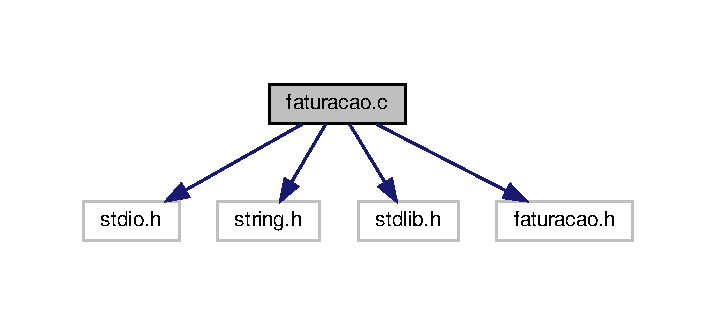
\includegraphics[width=344pt]{faturacao_8c__incl}
\end{center}
\end{figure}
\subsection*{Classes}
\begin{DoxyCompactItemize}
\item 
struct \hyperlink{structmes}{mes}
\item 
struct \hyperlink{structfil}{fil}
\item 
struct \hyperlink{structprd}{prd}
\item 
struct \hyperlink{structbucketv}{bucketv}
\item 
struct \hyperlink{structfat}{fat}
\end{DoxyCompactItemize}
\subsection*{Typedefs}
\begin{DoxyCompactItemize}
\item 
\mbox{\Hypertarget{faturacao_8c_ae69e537c5a1f6bd8bb80388ab93eaae8}\label{faturacao_8c_ae69e537c5a1f6bd8bb80388ab93eaae8}} 
typedef struct \hyperlink{structmes}{mes} {\bfseries Mes}
\item 
\mbox{\Hypertarget{faturacao_8c_ada38d1bc139c1d857a5829cf851da95d}\label{faturacao_8c_ada38d1bc139c1d857a5829cf851da95d}} 
typedef struct \hyperlink{structfil}{fil} {\bfseries Fil}
\item 
\mbox{\Hypertarget{faturacao_8c_abf8c3bb83510c329a4aef4eaafdde82c}\label{faturacao_8c_abf8c3bb83510c329a4aef4eaafdde82c}} 
typedef struct \hyperlink{structprd}{prd} {\bfseries Prd}
\item 
\mbox{\Hypertarget{faturacao_8c_a284dfffe5d015e87c0660e4f6cb349dc}\label{faturacao_8c_a284dfffe5d015e87c0660e4f6cb349dc}} 
typedef struct \hyperlink{structbucketv}{bucketv} {\bfseries Bucketv}
\item 
\mbox{\Hypertarget{faturacao_8c_ae353ee22d66ae2b54a25837375ee309d}\label{faturacao_8c_ae353ee22d66ae2b54a25837375ee309d}} 
typedef struct \hyperlink{structfat}{fat} {\bfseries Fat}
\end{DoxyCompactItemize}
\subsection*{Functions}
\begin{DoxyCompactItemize}
\item 
int \hyperlink{faturacao_8c_a173be3e70710c853405fe2e25ccf705a}{get\+Posicao\+Prod} (\hyperlink{structfat}{Fat} $\ast$\hyperlink{structfat}{fat}, char $\ast$product\+ID)
\begin{DoxyCompactList}\small\item\em Função que retorna o indice de um determinado produto da estrutura Fat. \end{DoxyCompactList}\item 
int \hyperlink{faturacao_8c_a004bfe584c9ee11a23c4e9f2630c091d}{get\+VendasN} (\hyperlink{structfat}{Fat} $\ast$\hyperlink{structfat}{fat}, int h, int pos, int m, int f)
\begin{DoxyCompactList}\small\item\em Função que retorna o numero de vendas em N de um terminado produto. \end{DoxyCompactList}\item 
int \hyperlink{faturacao_8c_ae9d0f03ab84c674b04f275a5084881c5}{get\+VendasP} (\hyperlink{structfat}{Fat} $\ast$\hyperlink{structfat}{fat}, int h, int pos, int m, int f)
\begin{DoxyCompactList}\small\item\em Função que retorna o numero de vendas em P de um terminado produto. \end{DoxyCompactList}\item 
double \hyperlink{faturacao_8c_a03449fad5aa8a7784ec140aa2d93604e}{get\+FaturacaoN} (\hyperlink{structfat}{Fat} $\ast$\hyperlink{structfat}{fat}, int h, int pos, int m, int f)
\begin{DoxyCompactList}\small\item\em Função que retorna a faturacao em N de um terminado produto. \end{DoxyCompactList}\item 
double \hyperlink{faturacao_8c_a4fe60cef21109a343cccf89de0195069}{get\+FaturacaoP} (\hyperlink{structfat}{Fat} $\ast$\hyperlink{structfat}{fat}, int h, int pos, int m, int f)
\begin{DoxyCompactList}\small\item\em Função que retorna a faturacao em P de um terminado produto. \end{DoxyCompactList}\item 
int \hyperlink{faturacao_8c_ac7b0f5071f35616572de14a725feb231}{get\+Size\+ArrayP} (\hyperlink{structfat}{Fat} $\ast$f, int key)
\begin{DoxyCompactList}\small\item\em Função que retorna o tamanho de um array num determinado indice da tabela. \end{DoxyCompactList}\item 
int \hyperlink{faturacao_8c_aaca35aa4a6d19ff7cd542a79d2f9676e}{get\+Filial\+Used} (\hyperlink{structfat}{Fat} $\ast$f, int key, int ip, int \hyperlink{structfil}{fil})
\begin{DoxyCompactList}\small\item\em Função que retorna se a filiaĺ foi \char`\"{}usada\char`\"{} ou não. \end{DoxyCompactList}\item 
char $\ast$ \hyperlink{faturacao_8c_ac4aecaf6413f812ff21c38d65928a33e}{get\+Prod\+Fat} (\hyperlink{structfat}{Fat} $\ast$f, int key, int ip)
\begin{DoxyCompactList}\small\item\em Função que retorna a string correspodente ao produto nos indices dados. \end{DoxyCompactList}\item 
int \hyperlink{faturacao_8c_ae7f12f7076e6f1faba71007c48f03247}{hashfat} (char $\ast$cont)
\begin{DoxyCompactList}\small\item\em Função que recebe uma string e subtrai ao primeiro elemnto da string a letra A. \end{DoxyCompactList}\item 
\hyperlink{structfat}{Fat} $\ast$ \hyperlink{faturacao_8c_ab9344ac52d509ff06cc1691365698508}{init\+Fat} ()
\begin{DoxyCompactList}\small\item\em Função que inicia uma estrutura Fat alocando espaço para todas as estruturas adjacentes. \end{DoxyCompactList}\item 
void \hyperlink{faturacao_8c_a04f1dcf92ec47d41d6e4b1e0529fdd89}{destroi\+Fat} (\hyperlink{structfat}{Fat} $\ast$f)
\begin{DoxyCompactList}\small\item\em Funçao que destroi uma estrutura Fat libertando o espaço ocupado por esta. \end{DoxyCompactList}\item 
void \hyperlink{faturacao_8c_a25accba27b71cf17ffb8ec42415526a9}{acrescenta\+\_\+prod} (\hyperlink{structfat}{Fat} $\ast$f, char $\ast$p)
\begin{DoxyCompactList}\small\item\em Função que acrescenta a uma Fat um produto. \end{DoxyCompactList}\item 
int \hyperlink{faturacao_8c_a0701ba6eeb7ce5a38b60552840603da3}{acrescenta\+\_\+prods} (\hyperlink{structfat}{Fat} $\ast$f, char $\ast$$\ast$p, int tam)
\begin{DoxyCompactList}\small\item\em Função que acrescenta a uma Fat vários produtos lidos de um array a strings. \end{DoxyCompactList}\item 
int \hyperlink{faturacao_8c_af4f597c733bfc2b1f31bdbcdf3932edb}{existe\+\_\+fat} (\hyperlink{structprd}{Prd} $\ast$arr, char $\ast$procurado, int Tam)
\begin{DoxyCompactList}\small\item\em Função que retorna o indice de um determinado produto da estrutura Fat caso ele exista -\/1 caso não. \end{DoxyCompactList}\item 
void \hyperlink{faturacao_8c_a5177262f2a6cf18a1f177fa11f0b8f4a}{acrescenta\+Fat} (\hyperlink{structfat}{Fat} $\ast$h, char $\ast$p, double pr, int q, char e, char $\ast$c, int m, int f)
\begin{DoxyCompactList}\small\item\em Função que acrescenta a uma Fat informação correspondente a um produto. \end{DoxyCompactList}\item 
char $\ast$$\ast$ \hyperlink{faturacao_8c_a1d6a7e597f26d5653f40d0a99d68d587}{never\+Bought\+Fil} (\hyperlink{structfat}{Fat} $\ast$f, int \hyperlink{structfil}{fil}, int $\ast$tamp)
\begin{DoxyCompactList}\small\item\em Função que retorna um array de strings com os produtos que nunca foram comprados numa filial em especifico. \end{DoxyCompactList}\item 
char $\ast$$\ast$ \hyperlink{faturacao_8c_a43d4ec277fadf56db60e03d14c294d92}{never\+Bought\+All\+Fil} (\hyperlink{structfat}{Fat} $\ast$f, int $\ast$tamp)
\begin{DoxyCompactList}\small\item\em Função que retorna um array de strings com os produtos que nunca foram comprados em nenhuma filial. \end{DoxyCompactList}\item 
int \hyperlink{faturacao_8c_af3b481b76c1fddff1bb6023ba36a094c}{Produtos\+Nao\+Comprados} (\hyperlink{structfat}{Fat} $\ast$f)
\begin{DoxyCompactList}\small\item\em Função que retorna o numero do produtos que nunca foram comprados. \end{DoxyCompactList}\item 
void \hyperlink{faturacao_8c_a985af7e60585c1c09340505c0bcd3185}{Faturacaoe\+Vendas\+Intervalo} (\hyperlink{structfat}{Fat} $\ast$f, int m1, int m2, int $\ast$result, double $\ast$result2)
\begin{DoxyCompactList}\small\item\em Função que retorna a faturacao(numero de vendas e faturado) num intervalo de meses. \end{DoxyCompactList}\end{DoxyCompactItemize}


\subsection{Detailed Description}
Modulo que contém as funcções para processamento, validação de faturas. 



\subsection{Function Documentation}
\mbox{\Hypertarget{faturacao_8c_a25accba27b71cf17ffb8ec42415526a9}\label{faturacao_8c_a25accba27b71cf17ffb8ec42415526a9}} 
\index{faturacao.\+c@{faturacao.\+c}!acrescenta\+\_\+prod@{acrescenta\+\_\+prod}}
\index{acrescenta\+\_\+prod@{acrescenta\+\_\+prod}!faturacao.\+c@{faturacao.\+c}}
\subsubsection{\texorpdfstring{acrescenta\+\_\+prod()}{acrescenta\_prod()}}
{\footnotesize\ttfamily void acrescenta\+\_\+prod (\begin{DoxyParamCaption}\item[{\hyperlink{structfat}{Fat} $\ast$}]{f,  }\item[{char $\ast$}]{p }\end{DoxyParamCaption})}



Função que acrescenta a uma Fat um produto. 

Aplicando a função hash descobre a posicao correta desta na Fat e sucessivamente realocando espaço para o adicionar á mesma


\begin{DoxyParams}{Parameters}
{\em Fat} & $\ast$f Fat previamente inicializada \\
\hline
{\em char} & $\ast$cont String genérica (produto) \\
\hline
\end{DoxyParams}
\mbox{\Hypertarget{faturacao_8c_a0701ba6eeb7ce5a38b60552840603da3}\label{faturacao_8c_a0701ba6eeb7ce5a38b60552840603da3}} 
\index{faturacao.\+c@{faturacao.\+c}!acrescenta\+\_\+prods@{acrescenta\+\_\+prods}}
\index{acrescenta\+\_\+prods@{acrescenta\+\_\+prods}!faturacao.\+c@{faturacao.\+c}}
\subsubsection{\texorpdfstring{acrescenta\+\_\+prods()}{acrescenta\_prods()}}
{\footnotesize\ttfamily int acrescenta\+\_\+prods (\begin{DoxyParamCaption}\item[{\hyperlink{structfat}{Fat} $\ast$}]{f,  }\item[{char $\ast$$\ast$}]{p,  }\item[{int}]{tam }\end{DoxyParamCaption})}



Função que acrescenta a uma Fat vários produtos lidos de um array a strings. 


\begin{DoxyParams}{Parameters}
{\em Fat} & $\ast$f Fat previamente inicializada \\
\hline
{\em char} & $\ast$$\ast$p Array de strings(produtos) \\
\hline
{\em int} & Tam Size do array de strings\\
\hline
\end{DoxyParams}
\begin{DoxyReturn}{Returns}
int i Numero de produtos acrescentados 
\end{DoxyReturn}
\mbox{\Hypertarget{faturacao_8c_a5177262f2a6cf18a1f177fa11f0b8f4a}\label{faturacao_8c_a5177262f2a6cf18a1f177fa11f0b8f4a}} 
\index{faturacao.\+c@{faturacao.\+c}!acrescenta\+Fat@{acrescenta\+Fat}}
\index{acrescenta\+Fat@{acrescenta\+Fat}!faturacao.\+c@{faturacao.\+c}}
\subsubsection{\texorpdfstring{acrescenta\+Fat()}{acrescentaFat()}}
{\footnotesize\ttfamily void acrescenta\+Fat (\begin{DoxyParamCaption}\item[{\hyperlink{structfat}{Fat} $\ast$}]{h,  }\item[{char $\ast$}]{p,  }\item[{double}]{pr,  }\item[{int}]{q,  }\item[{char}]{e,  }\item[{char $\ast$}]{c,  }\item[{int}]{m,  }\item[{int}]{f }\end{DoxyParamCaption})}



Função que acrescenta a uma Fat informação correspondente a um produto. 


\begin{DoxyParams}{Parameters}
{\em Fat} & $\ast$h Estrutua Fat \\
\hline
{\em char} & $\ast$p Produto \\
\hline
{\em double} & pr Preco \\
\hline
{\em int} & q Quantidade \\
\hline
{\em char} & e Modo de compra \\
\hline
{\em char} & $\ast$c Cliente \\
\hline
{\em int} & m Mes \\
\hline
{\em int} & f Filial \\
\hline
\end{DoxyParams}
\mbox{\Hypertarget{faturacao_8c_a04f1dcf92ec47d41d6e4b1e0529fdd89}\label{faturacao_8c_a04f1dcf92ec47d41d6e4b1e0529fdd89}} 
\index{faturacao.\+c@{faturacao.\+c}!destroi\+Fat@{destroi\+Fat}}
\index{destroi\+Fat@{destroi\+Fat}!faturacao.\+c@{faturacao.\+c}}
\subsubsection{\texorpdfstring{destroi\+Fat()}{destroiFat()}}
{\footnotesize\ttfamily void destroi\+Fat (\begin{DoxyParamCaption}\item[{\hyperlink{structfat}{Fat} $\ast$}]{f }\end{DoxyParamCaption})}



Funçao que destroi uma estrutura Fat libertando o espaço ocupado por esta. 


\begin{DoxyParams}{Parameters}
{\em Fat} & $\ast$f Fat previamente inicializada \\
\hline
\end{DoxyParams}
\mbox{\Hypertarget{faturacao_8c_af4f597c733bfc2b1f31bdbcdf3932edb}\label{faturacao_8c_af4f597c733bfc2b1f31bdbcdf3932edb}} 
\index{faturacao.\+c@{faturacao.\+c}!existe\+\_\+fat@{existe\+\_\+fat}}
\index{existe\+\_\+fat@{existe\+\_\+fat}!faturacao.\+c@{faturacao.\+c}}
\subsubsection{\texorpdfstring{existe\+\_\+fat()}{existe\_fat()}}
{\footnotesize\ttfamily int existe\+\_\+fat (\begin{DoxyParamCaption}\item[{\hyperlink{structprd}{Prd} $\ast$}]{arr,  }\item[{char $\ast$}]{procurado,  }\item[{int}]{Tam }\end{DoxyParamCaption})}



Função que retorna o indice de um determinado produto da estrutura Fat caso ele exista -\/1 caso não. 


\begin{DoxyParams}{Parameters}
{\em Prd} & $\ast$arr Array de Prd ( estrutura complementar de Fat) \\
\hline
{\em char} & $\ast$procurado Produto procurado \\
\hline
{\em int} & Tam Size do array de Prd\\
\hline
\end{DoxyParams}
\begin{DoxyReturn}{Returns}
int r Indice do produto se encontrado 
\end{DoxyReturn}
\mbox{\Hypertarget{faturacao_8c_a985af7e60585c1c09340505c0bcd3185}\label{faturacao_8c_a985af7e60585c1c09340505c0bcd3185}} 
\index{faturacao.\+c@{faturacao.\+c}!Faturacaoe\+Vendas\+Intervalo@{Faturacaoe\+Vendas\+Intervalo}}
\index{Faturacaoe\+Vendas\+Intervalo@{Faturacaoe\+Vendas\+Intervalo}!faturacao.\+c@{faturacao.\+c}}
\subsubsection{\texorpdfstring{Faturacaoe\+Vendas\+Intervalo()}{FaturacaoeVendasIntervalo()}}
{\footnotesize\ttfamily void Faturacaoe\+Vendas\+Intervalo (\begin{DoxyParamCaption}\item[{\hyperlink{structfat}{Fat} $\ast$}]{f,  }\item[{int}]{m1,  }\item[{int}]{m2,  }\item[{int $\ast$}]{result,  }\item[{double $\ast$}]{result2 }\end{DoxyParamCaption})}



Função que retorna a faturacao(numero de vendas e faturado) num intervalo de meses. 


\begin{DoxyParams}{Parameters}
{\em Fat} & $\ast$fat Estrutura Faturaçao \\
\hline
{\em int} & m1 Primeiro mes \\
\hline
{\em int} & m2 Segundo mes \\
\hline
{\em int} & $\ast$result Resultado a ser preenchido com o numero de vendas \\
\hline
{\em double} & $\ast$result2 Resultado a ser preenchido com o total faturado \\
\hline
\end{DoxyParams}
\mbox{\Hypertarget{faturacao_8c_a03449fad5aa8a7784ec140aa2d93604e}\label{faturacao_8c_a03449fad5aa8a7784ec140aa2d93604e}} 
\index{faturacao.\+c@{faturacao.\+c}!get\+FaturacaoN@{get\+FaturacaoN}}
\index{get\+FaturacaoN@{get\+FaturacaoN}!faturacao.\+c@{faturacao.\+c}}
\subsubsection{\texorpdfstring{get\+Faturacao\+N()}{getFaturacaoN()}}
{\footnotesize\ttfamily double get\+FaturacaoN (\begin{DoxyParamCaption}\item[{\hyperlink{structfat}{Fat} $\ast$}]{fat,  }\item[{int}]{h,  }\item[{int}]{pos,  }\item[{int}]{m,  }\item[{int}]{f }\end{DoxyParamCaption})}



Função que retorna a faturacao em N de um terminado produto. 


\begin{DoxyParams}{Parameters}
{\em Fat} & $\ast$fat Estrutura Faturaçao \\
\hline
{\em int} & h O indice do produto na tabela \\
\hline
{\em int} & pos O indice do produto dentro do seu respetivo array \\
\hline
{\em int} & m O indice do mes \\
\hline
{\em int} & f O indice da filial\\
\hline
\end{DoxyParams}
\begin{DoxyReturn}{Returns}
int Retorno do faturado em N 
\end{DoxyReturn}
\mbox{\Hypertarget{faturacao_8c_a4fe60cef21109a343cccf89de0195069}\label{faturacao_8c_a4fe60cef21109a343cccf89de0195069}} 
\index{faturacao.\+c@{faturacao.\+c}!get\+FaturacaoP@{get\+FaturacaoP}}
\index{get\+FaturacaoP@{get\+FaturacaoP}!faturacao.\+c@{faturacao.\+c}}
\subsubsection{\texorpdfstring{get\+Faturacao\+P()}{getFaturacaoP()}}
{\footnotesize\ttfamily double get\+FaturacaoP (\begin{DoxyParamCaption}\item[{\hyperlink{structfat}{Fat} $\ast$}]{fat,  }\item[{int}]{h,  }\item[{int}]{pos,  }\item[{int}]{m,  }\item[{int}]{f }\end{DoxyParamCaption})}



Função que retorna a faturacao em P de um terminado produto. 


\begin{DoxyParams}{Parameters}
{\em Fat} & $\ast$fat Estrutura Faturaçao \\
\hline
{\em int} & h O indice do produto na tabela \\
\hline
{\em int} & pos O indice do produto dentro do seu respetivo array \\
\hline
{\em int} & m O indice do mes \\
\hline
{\em int} & f O indice da filial\\
\hline
\end{DoxyParams}
\begin{DoxyReturn}{Returns}
int Retorno do faturado em P 
\end{DoxyReturn}
\mbox{\Hypertarget{faturacao_8c_aaca35aa4a6d19ff7cd542a79d2f9676e}\label{faturacao_8c_aaca35aa4a6d19ff7cd542a79d2f9676e}} 
\index{faturacao.\+c@{faturacao.\+c}!get\+Filial\+Used@{get\+Filial\+Used}}
\index{get\+Filial\+Used@{get\+Filial\+Used}!faturacao.\+c@{faturacao.\+c}}
\subsubsection{\texorpdfstring{get\+Filial\+Used()}{getFilialUsed()}}
{\footnotesize\ttfamily int get\+Filial\+Used (\begin{DoxyParamCaption}\item[{\hyperlink{structfat}{Fat} $\ast$}]{f,  }\item[{int}]{key,  }\item[{int}]{ip,  }\item[{int}]{fil }\end{DoxyParamCaption})}



Função que retorna se a filiaĺ foi \char`\"{}usada\char`\"{} ou não. 

Esta encontra-\/se usada se tiverem sido realizadas compras desse produto nessa filial


\begin{DoxyParams}{Parameters}
{\em Fat} & $\ast$fat Estrutura Faturaçao \\
\hline
{\em int} & key O indice do array na tabela \\
\hline
{\em int} & ip O indice do produto dentro do seu respetivo array \\
\hline
{\em int} & fil O indice da filial\\
\hline
\end{DoxyParams}
\begin{DoxyReturn}{Returns}
int Retorno do faturado em N 
\end{DoxyReturn}
\mbox{\Hypertarget{faturacao_8c_a173be3e70710c853405fe2e25ccf705a}\label{faturacao_8c_a173be3e70710c853405fe2e25ccf705a}} 
\index{faturacao.\+c@{faturacao.\+c}!get\+Posicao\+Prod@{get\+Posicao\+Prod}}
\index{get\+Posicao\+Prod@{get\+Posicao\+Prod}!faturacao.\+c@{faturacao.\+c}}
\subsubsection{\texorpdfstring{get\+Posicao\+Prod()}{getPosicaoProd()}}
{\footnotesize\ttfamily int get\+Posicao\+Prod (\begin{DoxyParamCaption}\item[{\hyperlink{structfat}{Fat} $\ast$}]{fat,  }\item[{char $\ast$}]{product\+ID }\end{DoxyParamCaption})}



Função que retorna o indice de um determinado produto da estrutura Fat. 


\begin{DoxyParams}{Parameters}
{\em Fat} & $\ast$fat Tabela de onde é retirado o cliente \\
\hline
{\em $\ast$product\+ID} & O produto a ser procurado\\
\hline
\end{DoxyParams}
\begin{DoxyReturn}{Returns}
int Retorno do indice deste na Fat 
\end{DoxyReturn}
\mbox{\Hypertarget{faturacao_8c_ac4aecaf6413f812ff21c38d65928a33e}\label{faturacao_8c_ac4aecaf6413f812ff21c38d65928a33e}} 
\index{faturacao.\+c@{faturacao.\+c}!get\+Prod\+Fat@{get\+Prod\+Fat}}
\index{get\+Prod\+Fat@{get\+Prod\+Fat}!faturacao.\+c@{faturacao.\+c}}
\subsubsection{\texorpdfstring{get\+Prod\+Fat()}{getProdFat()}}
{\footnotesize\ttfamily char$\ast$ get\+Prod\+Fat (\begin{DoxyParamCaption}\item[{\hyperlink{structfat}{Fat} $\ast$}]{f,  }\item[{int}]{key,  }\item[{int}]{ip }\end{DoxyParamCaption})}



Função que retorna a string correspodente ao produto nos indices dados. 


\begin{DoxyParams}{Parameters}
{\em Fat} & $\ast$fat Estrutura Faturaçao \\
\hline
{\em int} & key O indice do produto na tabela \\
\hline
{\em int} & ip O indice do produto dentro do seu respetivo array\\
\hline
\end{DoxyParams}
\begin{DoxyReturn}{Returns}
int Retorno do faturado em N 
\end{DoxyReturn}
\mbox{\Hypertarget{faturacao_8c_ac7b0f5071f35616572de14a725feb231}\label{faturacao_8c_ac7b0f5071f35616572de14a725feb231}} 
\index{faturacao.\+c@{faturacao.\+c}!get\+Size\+ArrayP@{get\+Size\+ArrayP}}
\index{get\+Size\+ArrayP@{get\+Size\+ArrayP}!faturacao.\+c@{faturacao.\+c}}
\subsubsection{\texorpdfstring{get\+Size\+Array\+P()}{getSizeArrayP()}}
{\footnotesize\ttfamily int get\+Size\+ArrayP (\begin{DoxyParamCaption}\item[{\hyperlink{structfat}{Fat} $\ast$}]{f,  }\item[{int}]{key }\end{DoxyParamCaption})}



Função que retorna o tamanho de um array num determinado indice da tabela. 


\begin{DoxyParams}{Parameters}
{\em Fat} & $\ast$fat Estrutura Faturaçao \\
\hline
{\em int} & key O indice do arr na tabela\\
\hline
\end{DoxyParams}
\begin{DoxyReturn}{Returns}
int Retorno do size do array 
\end{DoxyReturn}
\mbox{\Hypertarget{faturacao_8c_a004bfe584c9ee11a23c4e9f2630c091d}\label{faturacao_8c_a004bfe584c9ee11a23c4e9f2630c091d}} 
\index{faturacao.\+c@{faturacao.\+c}!get\+VendasN@{get\+VendasN}}
\index{get\+VendasN@{get\+VendasN}!faturacao.\+c@{faturacao.\+c}}
\subsubsection{\texorpdfstring{get\+Vendas\+N()}{getVendasN()}}
{\footnotesize\ttfamily int get\+VendasN (\begin{DoxyParamCaption}\item[{\hyperlink{structfat}{Fat} $\ast$}]{fat,  }\item[{int}]{h,  }\item[{int}]{pos,  }\item[{int}]{m,  }\item[{int}]{f }\end{DoxyParamCaption})}



Função que retorna o numero de vendas em N de um terminado produto. 


\begin{DoxyParams}{Parameters}
{\em Fat} & $\ast$fat Estrutura Faturaçao \\
\hline
{\em int} & h O indice do produto na tabela \\
\hline
{\em int} & pos O indice do produto dentro do seu respetivo array \\
\hline
{\em int} & m O indice do mes \\
\hline
{\em int} & f O indice da filial\\
\hline
\end{DoxyParams}
\begin{DoxyReturn}{Returns}
int Retorno do numero de vendas em N 
\end{DoxyReturn}
\mbox{\Hypertarget{faturacao_8c_ae9d0f03ab84c674b04f275a5084881c5}\label{faturacao_8c_ae9d0f03ab84c674b04f275a5084881c5}} 
\index{faturacao.\+c@{faturacao.\+c}!get\+VendasP@{get\+VendasP}}
\index{get\+VendasP@{get\+VendasP}!faturacao.\+c@{faturacao.\+c}}
\subsubsection{\texorpdfstring{get\+Vendas\+P()}{getVendasP()}}
{\footnotesize\ttfamily int get\+VendasP (\begin{DoxyParamCaption}\item[{\hyperlink{structfat}{Fat} $\ast$}]{fat,  }\item[{int}]{h,  }\item[{int}]{pos,  }\item[{int}]{m,  }\item[{int}]{f }\end{DoxyParamCaption})}



Função que retorna o numero de vendas em P de um terminado produto. 


\begin{DoxyParams}{Parameters}
{\em Fat} & $\ast$fat Estrutura Faturaçao \\
\hline
{\em int} & h O indice do produto na tabela \\
\hline
{\em int} & pos O indice do produto dentro do seu respetivo array \\
\hline
{\em int} & m O indice do mes \\
\hline
{\em int} & f O indice da filial\\
\hline
\end{DoxyParams}
\begin{DoxyReturn}{Returns}
int Retorno do numero de vendas em P 
\end{DoxyReturn}
\mbox{\Hypertarget{faturacao_8c_ae7f12f7076e6f1faba71007c48f03247}\label{faturacao_8c_ae7f12f7076e6f1faba71007c48f03247}} 
\index{faturacao.\+c@{faturacao.\+c}!hashfat@{hashfat}}
\index{hashfat@{hashfat}!faturacao.\+c@{faturacao.\+c}}
\subsubsection{\texorpdfstring{hashfat()}{hashfat()}}
{\footnotesize\ttfamily int hashfat (\begin{DoxyParamCaption}\item[{char $\ast$}]{cont }\end{DoxyParamCaption})}



Função que recebe uma string e subtrai ao primeiro elemnto da string a letra A. 


\begin{DoxyParams}{Parameters}
{\em char} & $\ast$cont String genérica\\
\hline
\end{DoxyParams}
\begin{DoxyReturn}{Returns}
int O resultado inteiro dessa subtração 
\end{DoxyReturn}
\mbox{\Hypertarget{faturacao_8c_ab9344ac52d509ff06cc1691365698508}\label{faturacao_8c_ab9344ac52d509ff06cc1691365698508}} 
\index{faturacao.\+c@{faturacao.\+c}!init\+Fat@{init\+Fat}}
\index{init\+Fat@{init\+Fat}!faturacao.\+c@{faturacao.\+c}}
\subsubsection{\texorpdfstring{init\+Fat()}{initFat()}}
{\footnotesize\ttfamily \hyperlink{structfat}{Fat}$\ast$ init\+Fat (\begin{DoxyParamCaption}{ }\end{DoxyParamCaption})}



Função que inicia uma estrutura Fat alocando espaço para todas as estruturas adjacentes. 

\begin{DoxyReturn}{Returns}
Fat$\ast$ Devolve a Fat inicializada 
\end{DoxyReturn}
\mbox{\Hypertarget{faturacao_8c_a43d4ec277fadf56db60e03d14c294d92}\label{faturacao_8c_a43d4ec277fadf56db60e03d14c294d92}} 
\index{faturacao.\+c@{faturacao.\+c}!never\+Bought\+All\+Fil@{never\+Bought\+All\+Fil}}
\index{never\+Bought\+All\+Fil@{never\+Bought\+All\+Fil}!faturacao.\+c@{faturacao.\+c}}
\subsubsection{\texorpdfstring{never\+Bought\+All\+Fil()}{neverBoughtAllFil()}}
{\footnotesize\ttfamily char$\ast$$\ast$ never\+Bought\+All\+Fil (\begin{DoxyParamCaption}\item[{\hyperlink{structfat}{Fat} $\ast$}]{f,  }\item[{int $\ast$}]{tamp }\end{DoxyParamCaption})}



Função que retorna um array de strings com os produtos que nunca foram comprados em nenhuma filial. 


\begin{DoxyParams}{Parameters}
{\em Fat} & $\ast$fat Estrutura Faturaçao \\
\hline
{\em int} & tamp um size que a função vai alterar\\
\hline
\end{DoxyParams}
\begin{DoxyReturn}{Returns}
char$\ast$$\ast$ array de strings com os produtos 
\end{DoxyReturn}
\mbox{\Hypertarget{faturacao_8c_a1d6a7e597f26d5653f40d0a99d68d587}\label{faturacao_8c_a1d6a7e597f26d5653f40d0a99d68d587}} 
\index{faturacao.\+c@{faturacao.\+c}!never\+Bought\+Fil@{never\+Bought\+Fil}}
\index{never\+Bought\+Fil@{never\+Bought\+Fil}!faturacao.\+c@{faturacao.\+c}}
\subsubsection{\texorpdfstring{never\+Bought\+Fil()}{neverBoughtFil()}}
{\footnotesize\ttfamily char$\ast$$\ast$ never\+Bought\+Fil (\begin{DoxyParamCaption}\item[{\hyperlink{structfat}{Fat} $\ast$}]{f,  }\item[{int}]{fil,  }\item[{int $\ast$}]{tamp }\end{DoxyParamCaption})}



Função que retorna um array de strings com os produtos que nunca foram comprados numa filial em especifico. 


\begin{DoxyParams}{Parameters}
{\em Fat} & $\ast$fat Estrutura Faturaçao \\
\hline
{\em int} & fil Filial \\
\hline
{\em int} & tamp um size que a função vai alterar\\
\hline
\end{DoxyParams}
\begin{DoxyReturn}{Returns}
char$\ast$$\ast$ array de strings com os produtos 
\end{DoxyReturn}
\mbox{\Hypertarget{faturacao_8c_af3b481b76c1fddff1bb6023ba36a094c}\label{faturacao_8c_af3b481b76c1fddff1bb6023ba36a094c}} 
\index{faturacao.\+c@{faturacao.\+c}!Produtos\+Nao\+Comprados@{Produtos\+Nao\+Comprados}}
\index{Produtos\+Nao\+Comprados@{Produtos\+Nao\+Comprados}!faturacao.\+c@{faturacao.\+c}}
\subsubsection{\texorpdfstring{Produtos\+Nao\+Comprados()}{ProdutosNaoComprados()}}
{\footnotesize\ttfamily int Produtos\+Nao\+Comprados (\begin{DoxyParamCaption}\item[{\hyperlink{structfat}{Fat} $\ast$}]{f }\end{DoxyParamCaption})}



Função que retorna o numero do produtos que nunca foram comprados. 


\begin{DoxyParams}{Parameters}
{\em Fat} & $\ast$fat Estrutura Faturaçao\\
\hline
\end{DoxyParams}
\begin{DoxyReturn}{Returns}
int Numero de produtos nunca comprados 
\end{DoxyReturn}

\hypertarget{filiais_8c}{}\section{filiais.\+c File Reference}
\label{filiais_8c}\index{filiais.\+c@{filiais.\+c}}


Modulo que contém as funcções para a gestão das filiais.  


{\ttfamily \#include $<$stdio.\+h$>$}\newline
{\ttfamily \#include $<$string.\+h$>$}\newline
{\ttfamily \#include $<$stdlib.\+h$>$}\newline
{\ttfamily \#include \char`\"{}filiais.\+h\char`\"{}}\newline
Include dependency graph for filiais.\+c\+:
\nopagebreak
\begin{figure}[H]
\begin{center}
\leavevmode
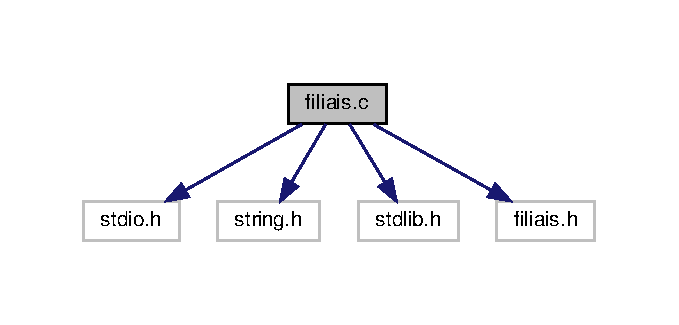
\includegraphics[width=326pt]{filiais_8c__incl}
\end{center}
\end{figure}
\subsection*{Classes}
\begin{DoxyCompactItemize}
\item 
struct \hyperlink{structqprd}{qprd}
\item 
struct \hyperlink{structmesf}{mesf}
\item 
struct \hyperlink{structfili}{fili}
\item 
struct \hyperlink{structcl}{cl}
\item 
struct \hyperlink{structbucketf}{bucketf}
\item 
struct \hyperlink{structfilial}{filial}
\end{DoxyCompactItemize}
\subsection*{Typedefs}
\begin{DoxyCompactItemize}
\item 
\mbox{\Hypertarget{filiais_8c_adf857ba1e38a54d1305eba5c62d8213b}\label{filiais_8c_adf857ba1e38a54d1305eba5c62d8213b}} 
typedef struct \hyperlink{structqprd}{qprd} {\bfseries Qprd}
\item 
\mbox{\Hypertarget{filiais_8c_af99564d83469f3d24b6fa99ced9c94f5}\label{filiais_8c_af99564d83469f3d24b6fa99ced9c94f5}} 
typedef struct \hyperlink{structmesf}{mesf} {\bfseries Mesf}
\item 
\mbox{\Hypertarget{filiais_8c_a4c6f8aff83c03b31765e15e33dcdace3}\label{filiais_8c_a4c6f8aff83c03b31765e15e33dcdace3}} 
typedef struct \hyperlink{structfili}{fili} {\bfseries Fili}
\item 
\mbox{\Hypertarget{filiais_8c_a5d55d8b4b787dd35a72e4ff5fc189b70}\label{filiais_8c_a5d55d8b4b787dd35a72e4ff5fc189b70}} 
typedef struct \hyperlink{structcl}{cl} {\bfseries Cl}
\item 
\mbox{\Hypertarget{filiais_8c_a688d98bbf4eb00e0ed7dd38f5b5ace00}\label{filiais_8c_a688d98bbf4eb00e0ed7dd38f5b5ace00}} 
typedef struct \hyperlink{structbucketf}{bucketf} {\bfseries Bucketf}
\item 
\mbox{\Hypertarget{filiais_8c_a93c8ad434fb99daf8769d6c0808c80d0}\label{filiais_8c_a93c8ad434fb99daf8769d6c0808c80d0}} 
typedef struct \hyperlink{structfilial}{filial} {\bfseries Filial}
\end{DoxyCompactItemize}
\subsection*{Functions}
\begin{DoxyCompactItemize}
\item 
int \hyperlink{filiais_8c_a48076566c412a2d179d2143381d4cd56}{get\+Fil\+Used} (\hyperlink{structfilial}{Filial} $\ast$f, int k, int ip, int \hyperlink{structfil}{fil})
\begin{DoxyCompactList}\small\item\em Função que verifica se uma filial é usada. \end{DoxyCompactList}\item 
char $\ast$ \hyperlink{filiais_8c_a2ae1ae9a1c4c47c395e7fa84137f6d02}{get\+C\+Liente} (\hyperlink{structfilial}{Filial} $\ast$f, int k, int ip)
\begin{DoxyCompactList}\small\item\em Função que devolve um cliente. \end{DoxyCompactList}\item 
int \hyperlink{filiais_8c_a312e754d04669008f7e6337f1d4d0ad2}{get\+Size\+Arr\+Client} (\hyperlink{structfilial}{Filial} $\ast$f, int k)
\begin{DoxyCompactList}\small\item\em Função que devolve o tamanho do array num determinado indice da tabela. \end{DoxyCompactList}\item 
\hyperlink{structcl}{Cl} $\ast$ \hyperlink{filiais_8c_abe257a0cf5a8f5b9ca16d917b1fc4462}{get\+Arr\+By\+Letter} (\hyperlink{structfilial}{Filial} $\ast$f, int key)
\begin{DoxyCompactList}\small\item\em Função que devolve um array de clientes começados por uma determinada letra. \end{DoxyCompactList}\item 
int \hyperlink{filiais_8c_aad712e4c0c4b04cdd8a1fde9a6d76960}{get\+Size\+Qprd} (\hyperlink{structfilial}{Filial} $\ast$f, int k, int id, int \hyperlink{structfil}{fil}, int m)
\begin{DoxyCompactList}\small\item\em Função que devolve o tamanho do array de produtos num determinado mês. \end{DoxyCompactList}\item 
int \hyperlink{filiais_8c_a5afbe4f63968b3973e03805a80e26538}{get\+QuantN} (\hyperlink{structfilial}{Filial} $\ast$f, int k, int id, int \hyperlink{structfil}{fil}, int m, int pid)
\begin{DoxyCompactList}\small\item\em Função que devolve q quantidade de compras em N para um determinado produto num mês. \end{DoxyCompactList}\item 
int \hyperlink{filiais_8c_ae2595ef550326e0f6fa7fa588280b8bc}{get\+QuantP} (\hyperlink{structfilial}{Filial} $\ast$f, int k, int id, int \hyperlink{structfil}{fil}, int m, int pid)
\begin{DoxyCompactList}\small\item\em Função que devolve a quantidade de compras em P para um determinado produto num mês. \end{DoxyCompactList}\item 
int \hyperlink{filiais_8c_a6041be59c26942021a4d770847ff57b1}{get\+GastoP} (\hyperlink{structfilial}{Filial} $\ast$f, int k, int id, int \hyperlink{structfil}{fil}, int m, int pid)
\begin{DoxyCompactList}\small\item\em Função que devolve gasto total em P de um determinado produto. \end{DoxyCompactList}\item 
int \hyperlink{filiais_8c_ac0951f8550239d484198d66a91d4d669}{get\+GastoN} (\hyperlink{structfilial}{Filial} $\ast$f, int k, int id, int \hyperlink{structfil}{fil}, int m, int pid)
\begin{DoxyCompactList}\small\item\em Função que devolve o gasto total em N de um determinado produto. \end{DoxyCompactList}\item 
char $\ast$ \hyperlink{filiais_8c_a040f730a447e54dababcf1465c416612}{get\+One\+Prod} (\hyperlink{structfilial}{Filial} $\ast$f, int k, int id, int \hyperlink{structfil}{fil}, int m, int p)
\begin{DoxyCompactList}\small\item\em Função que devolve um produto. \end{DoxyCompactList}\item 
int \hyperlink{filiais_8c_a8395dbae061751c7cf2ff01a8848cb4d}{hashfil} (char $\ast$cont)
\begin{DoxyCompactList}\small\item\em Função que recebe uma string e subtrai ao primeiro elemnto da string a letra A. \end{DoxyCompactList}\item 
\hyperlink{structfilial}{Filial} $\ast$ \hyperlink{filiais_8c_a5727000000ceab10ee0e17bcad54b96e}{init\+Filial} ()
\begin{DoxyCompactList}\small\item\em Função que inicia uma estrutura Filial alocando espaço para todas as estruturas adjacentes. \end{DoxyCompactList}\item 
void \hyperlink{filiais_8c_a05ef376e7b641cb197501af272c65ed8}{destroi\+Filial} (\hyperlink{structfilial}{Filial} $\ast$f)
\begin{DoxyCompactList}\small\item\em Funçao que destroi uma estrutura Filial libertando o espaço ocupado por esta. \end{DoxyCompactList}\item 
void \hyperlink{filiais_8c_a3e289644b4dfeedcbaced74babd68d94}{acrescenta\+\_\+cl} (\hyperlink{structfilial}{Filial} $\ast$f, char $\ast$p)
\begin{DoxyCompactList}\small\item\em Função que acrescenta a uma Filial um cliente. \end{DoxyCompactList}\item 
int \hyperlink{filiais_8c_a3ead5857287f11974aed18a3cc84fe8d}{acrescenta\+\_\+cls} (\hyperlink{structfilial}{Filial} $\ast$f, char $\ast$$\ast$p, int tam)
\begin{DoxyCompactList}\small\item\em Função que acrescenta a uma Filial vários clientes lidos de um array a strings. \end{DoxyCompactList}\item 
int \hyperlink{filiais_8c_a2d285c6f23a822150012d74bf0f4daa1}{existe\+\_\+fil} (\hyperlink{structcl}{Cl} $\ast$arr, char $\ast$procurado, int Tam)
\begin{DoxyCompactList}\small\item\em Função que retorna o indice de um determinado cliente da estrutura Filial caso ele exista, -\/1 caso não. \end{DoxyCompactList}\item 
int \hyperlink{filiais_8c_a7ed66b6cb4bb6dfb5ed5614e8051c11b}{existe\+\_\+prod} (\hyperlink{structqprd}{Qprd} $\ast$arr, char $\ast$procurado, int Tam)
\begin{DoxyCompactList}\small\item\em Função que retorna o indice de um determinado produto de um cliente caso ele exista, -\/1 caso não. \end{DoxyCompactList}\item 
void \hyperlink{filiais_8c_a62b9915663f5cd3a9cb514dba8e36cdd}{acrescenta\+Pto\+Fil} (\hyperlink{structfilial}{Filial} $\ast$h, char $\ast$p, int it, int a, int f, int m, char e, int qnt, int preco)
\begin{DoxyCompactList}\small\item\em Função que acrescenta um produto a um cliente na Filial. \end{DoxyCompactList}\item 
void \hyperlink{filiais_8c_afaa3aea9b4bfce86672dffc562720c02}{acrescenta\+Fil} (\hyperlink{structfilial}{Filial} $\ast$h, char $\ast$p, double pr, int q, char e, char $\ast$c, int m, int f)
\begin{DoxyCompactList}\small\item\em Função que acrescenta um produto a um cliente na Filial. \end{DoxyCompactList}\item 
char $\ast$$\ast$ \hyperlink{filiais_8c_a114a40a9fda2a951bdca3da1d135e9a3}{Clients\+Of\+All\+Branches} (\hyperlink{structfilial}{Filial} $\ast$f, int $\ast$tam)
\begin{DoxyCompactList}\small\item\em Função que retorna um array de strings com os clientes que compraram em todas as filiais. \end{DoxyCompactList}\item 
int \hyperlink{filiais_8c_a2f6bb55313708fcdd16e793e116f849b}{Clientes\+Sem\+Compras} (\hyperlink{structfilial}{Filial} $\ast$f)
\begin{DoxyCompactList}\small\item\em Função que retorna um array de strings com os clientes que nunca fizeram compras. \end{DoxyCompactList}\item 
int \hyperlink{filiais_8c_a35dcf3b835d306278e0d6a21e54b9b5f}{Quantidades\+Um\+Cliente\+Por\+Mes} (\hyperlink{structfilial}{Filial} $\ast$f, char $\ast$cliente\+ID, int \hyperlink{structfil}{fil}, int \hyperlink{structmes}{mes})
\begin{DoxyCompactList}\small\item\em Função que retorna a quantidade total de produtos comprados num mês. \end{DoxyCompactList}\end{DoxyCompactItemize}


\subsection{Detailed Description}
Modulo que contém as funcções para a gestão das filiais. 



\subsection{Function Documentation}
\mbox{\Hypertarget{filiais_8c_a3e289644b4dfeedcbaced74babd68d94}\label{filiais_8c_a3e289644b4dfeedcbaced74babd68d94}} 
\index{filiais.\+c@{filiais.\+c}!acrescenta\+\_\+cl@{acrescenta\+\_\+cl}}
\index{acrescenta\+\_\+cl@{acrescenta\+\_\+cl}!filiais.\+c@{filiais.\+c}}
\subsubsection{\texorpdfstring{acrescenta\+\_\+cl()}{acrescenta\_cl()}}
{\footnotesize\ttfamily void acrescenta\+\_\+cl (\begin{DoxyParamCaption}\item[{\hyperlink{structfilial}{Filial} $\ast$}]{f,  }\item[{char $\ast$}]{p }\end{DoxyParamCaption})}



Função que acrescenta a uma Filial um cliente. 

Aplicando a função hash descobre a posicao correta desta na Filial e sucessivamente realocando espaço para o adicionar á mesma


\begin{DoxyParams}{Parameters}
{\em Filial} & $\ast$f Fat previamente inicializada \\
\hline
{\em char} & $\ast$p String genérica (cliente) \\
\hline
\end{DoxyParams}
\mbox{\Hypertarget{filiais_8c_a3ead5857287f11974aed18a3cc84fe8d}\label{filiais_8c_a3ead5857287f11974aed18a3cc84fe8d}} 
\index{filiais.\+c@{filiais.\+c}!acrescenta\+\_\+cls@{acrescenta\+\_\+cls}}
\index{acrescenta\+\_\+cls@{acrescenta\+\_\+cls}!filiais.\+c@{filiais.\+c}}
\subsubsection{\texorpdfstring{acrescenta\+\_\+cls()}{acrescenta\_cls()}}
{\footnotesize\ttfamily int acrescenta\+\_\+cls (\begin{DoxyParamCaption}\item[{\hyperlink{structfilial}{Filial} $\ast$}]{f,  }\item[{char $\ast$$\ast$}]{p,  }\item[{int}]{tam }\end{DoxyParamCaption})}



Função que acrescenta a uma Filial vários clientes lidos de um array a strings. 


\begin{DoxyParams}{Parameters}
{\em Filial} & $\ast$f Filial previamente inicializada \\
\hline
{\em char} & $\ast$$\ast$p Array de strings(clientes) \\
\hline
{\em int} & Tam Size do array de strings\\
\hline
\end{DoxyParams}
\begin{DoxyReturn}{Returns}
int i Número de clientes acrescentados 
\end{DoxyReturn}
\mbox{\Hypertarget{filiais_8c_afaa3aea9b4bfce86672dffc562720c02}\label{filiais_8c_afaa3aea9b4bfce86672dffc562720c02}} 
\index{filiais.\+c@{filiais.\+c}!acrescenta\+Fil@{acrescenta\+Fil}}
\index{acrescenta\+Fil@{acrescenta\+Fil}!filiais.\+c@{filiais.\+c}}
\subsubsection{\texorpdfstring{acrescenta\+Fil()}{acrescentaFil()}}
{\footnotesize\ttfamily void acrescenta\+Fil (\begin{DoxyParamCaption}\item[{\hyperlink{structfilial}{Filial} $\ast$}]{h,  }\item[{char $\ast$}]{p,  }\item[{double}]{pr,  }\item[{int}]{q,  }\item[{char}]{e,  }\item[{char $\ast$}]{c,  }\item[{int}]{m,  }\item[{int}]{f }\end{DoxyParamCaption})}



Função que acrescenta um produto a um cliente na Filial. 


\begin{DoxyParams}{Parameters}
{\em Filial} & $\ast$h Estrutua Filial \\
\hline
{\em char} & $\ast$p Produto \\
\hline
{\em double} & pr Preço \\
\hline
{\em int} & q Quantidade \\
\hline
{\em char} & e Modo de compra \\
\hline
{\em char} & $\ast$c Cliente \\
\hline
{\em int} & m Mes \\
\hline
{\em int} & f Filial \\
\hline
\end{DoxyParams}
\mbox{\Hypertarget{filiais_8c_a62b9915663f5cd3a9cb514dba8e36cdd}\label{filiais_8c_a62b9915663f5cd3a9cb514dba8e36cdd}} 
\index{filiais.\+c@{filiais.\+c}!acrescenta\+Pto\+Fil@{acrescenta\+Pto\+Fil}}
\index{acrescenta\+Pto\+Fil@{acrescenta\+Pto\+Fil}!filiais.\+c@{filiais.\+c}}
\subsubsection{\texorpdfstring{acrescenta\+Pto\+Fil()}{acrescentaPtoFil()}}
{\footnotesize\ttfamily void acrescenta\+Pto\+Fil (\begin{DoxyParamCaption}\item[{\hyperlink{structfilial}{Filial} $\ast$}]{h,  }\item[{char $\ast$}]{p,  }\item[{int}]{it,  }\item[{int}]{a,  }\item[{int}]{f,  }\item[{int}]{m,  }\item[{char}]{e,  }\item[{int}]{qnt,  }\item[{int}]{preco }\end{DoxyParamCaption})}



Função que acrescenta um produto a um cliente na Filial. 


\begin{DoxyParams}{Parameters}
{\em Filial} & $\ast$h Estrutua Filial \\
\hline
{\em char} & $\ast$p Produto \\
\hline
{\em int} & it Indice do cliente na tabela \\
\hline
{\em int} & a Indice do cliente no array \\
\hline
{\em int} & f Filial \\
\hline
{\em int} & m Mes \\
\hline
{\em char} & e Modo de compra \\
\hline
{\em int} & qnt Quantidade \\
\hline
{\em int} & preco Preço \\
\hline
\end{DoxyParams}
\mbox{\Hypertarget{filiais_8c_a2f6bb55313708fcdd16e793e116f849b}\label{filiais_8c_a2f6bb55313708fcdd16e793e116f849b}} 
\index{filiais.\+c@{filiais.\+c}!Clientes\+Sem\+Compras@{Clientes\+Sem\+Compras}}
\index{Clientes\+Sem\+Compras@{Clientes\+Sem\+Compras}!filiais.\+c@{filiais.\+c}}
\subsubsection{\texorpdfstring{Clientes\+Sem\+Compras()}{ClientesSemCompras()}}
{\footnotesize\ttfamily int Clientes\+Sem\+Compras (\begin{DoxyParamCaption}\item[{\hyperlink{structfilial}{Filial} $\ast$}]{f }\end{DoxyParamCaption})}



Função que retorna um array de strings com os clientes que nunca fizeram compras. 


\begin{DoxyParams}{Parameters}
{\em Filial} & $\ast$f Estrutura Filial\\
\hline
\end{DoxyParams}
\begin{DoxyReturn}{Returns}
char$\ast$$\ast$ array de strings com os clientes 
\end{DoxyReturn}
\mbox{\Hypertarget{filiais_8c_a114a40a9fda2a951bdca3da1d135e9a3}\label{filiais_8c_a114a40a9fda2a951bdca3da1d135e9a3}} 
\index{filiais.\+c@{filiais.\+c}!Clients\+Of\+All\+Branches@{Clients\+Of\+All\+Branches}}
\index{Clients\+Of\+All\+Branches@{Clients\+Of\+All\+Branches}!filiais.\+c@{filiais.\+c}}
\subsubsection{\texorpdfstring{Clients\+Of\+All\+Branches()}{ClientsOfAllBranches()}}
{\footnotesize\ttfamily char$\ast$$\ast$ Clients\+Of\+All\+Branches (\begin{DoxyParamCaption}\item[{\hyperlink{structfilial}{Filial} $\ast$}]{f,  }\item[{int $\ast$}]{tam }\end{DoxyParamCaption})}



Função que retorna um array de strings com os clientes que compraram em todas as filiais. 


\begin{DoxyParams}{Parameters}
{\em Filial} & $\ast$f Estrutura Filial \\
\hline
{\em int} & $\ast$tam Um size que a função vai alterar\\
\hline
\end{DoxyParams}
\begin{DoxyReturn}{Returns}
char$\ast$$\ast$ array de strings com os clientes 
\end{DoxyReturn}
\mbox{\Hypertarget{filiais_8c_a05ef376e7b641cb197501af272c65ed8}\label{filiais_8c_a05ef376e7b641cb197501af272c65ed8}} 
\index{filiais.\+c@{filiais.\+c}!destroi\+Filial@{destroi\+Filial}}
\index{destroi\+Filial@{destroi\+Filial}!filiais.\+c@{filiais.\+c}}
\subsubsection{\texorpdfstring{destroi\+Filial()}{destroiFilial()}}
{\footnotesize\ttfamily void destroi\+Filial (\begin{DoxyParamCaption}\item[{\hyperlink{structfilial}{Filial} $\ast$}]{f }\end{DoxyParamCaption})}



Funçao que destroi uma estrutura Filial libertando o espaço ocupado por esta. 


\begin{DoxyParams}{Parameters}
{\em Filial} & $\ast$f Filial previamente inicializada \\
\hline
\end{DoxyParams}
\mbox{\Hypertarget{filiais_8c_a2d285c6f23a822150012d74bf0f4daa1}\label{filiais_8c_a2d285c6f23a822150012d74bf0f4daa1}} 
\index{filiais.\+c@{filiais.\+c}!existe\+\_\+fil@{existe\+\_\+fil}}
\index{existe\+\_\+fil@{existe\+\_\+fil}!filiais.\+c@{filiais.\+c}}
\subsubsection{\texorpdfstring{existe\+\_\+fil()}{existe\_fil()}}
{\footnotesize\ttfamily int existe\+\_\+fil (\begin{DoxyParamCaption}\item[{\hyperlink{structcl}{Cl} $\ast$}]{arr,  }\item[{char $\ast$}]{procurado,  }\item[{int}]{Tam }\end{DoxyParamCaption})}



Função que retorna o indice de um determinado cliente da estrutura Filial caso ele exista, -\/1 caso não. 


\begin{DoxyParams}{Parameters}
{\em Cl} & $\ast$arr Array de Cl ( estrutura complementar de Filial) \\
\hline
{\em char} & $\ast$procurado Cliente procurado \\
\hline
{\em int} & Tam Size do array de Cl\\
\hline
\end{DoxyParams}
\begin{DoxyReturn}{Returns}
int r Indice do cliente se encontrado 
\end{DoxyReturn}
\mbox{\Hypertarget{filiais_8c_a7ed66b6cb4bb6dfb5ed5614e8051c11b}\label{filiais_8c_a7ed66b6cb4bb6dfb5ed5614e8051c11b}} 
\index{filiais.\+c@{filiais.\+c}!existe\+\_\+prod@{existe\+\_\+prod}}
\index{existe\+\_\+prod@{existe\+\_\+prod}!filiais.\+c@{filiais.\+c}}
\subsubsection{\texorpdfstring{existe\+\_\+prod()}{existe\_prod()}}
{\footnotesize\ttfamily int existe\+\_\+prod (\begin{DoxyParamCaption}\item[{\hyperlink{structqprd}{Qprd} $\ast$}]{arr,  }\item[{char $\ast$}]{procurado,  }\item[{int}]{Tam }\end{DoxyParamCaption})}



Função que retorna o indice de um determinado produto de um cliente caso ele exista, -\/1 caso não. 


\begin{DoxyParams}{Parameters}
{\em Qprd} & $\ast$arr Array de Qprd ( estrutura complementar de Filial) \\
\hline
{\em char} & $\ast$procurado Produto procurado \\
\hline
{\em int} & Tam Size do array de Qprod\\
\hline
\end{DoxyParams}
\begin{DoxyReturn}{Returns}
int r Indice do produto se encontrado 
\end{DoxyReturn}
\mbox{\Hypertarget{filiais_8c_abe257a0cf5a8f5b9ca16d917b1fc4462}\label{filiais_8c_abe257a0cf5a8f5b9ca16d917b1fc4462}} 
\index{filiais.\+c@{filiais.\+c}!get\+Arr\+By\+Letter@{get\+Arr\+By\+Letter}}
\index{get\+Arr\+By\+Letter@{get\+Arr\+By\+Letter}!filiais.\+c@{filiais.\+c}}
\subsubsection{\texorpdfstring{get\+Arr\+By\+Letter()}{getArrByLetter()}}
{\footnotesize\ttfamily \hyperlink{structcl}{Cl}$\ast$ get\+Arr\+By\+Letter (\begin{DoxyParamCaption}\item[{\hyperlink{structfilial}{Filial} $\ast$}]{f,  }\item[{int}]{key }\end{DoxyParamCaption})}



Função que devolve um array de clientes começados por uma determinada letra. 


\begin{DoxyParams}{Parameters}
{\em Filial} & $\ast$f Estrutura filiais \\
\hline
{\em int} & k Indice do cliente na tabela \\
\hline
\end{DoxyParams}
\begin{DoxyReturn}{Returns}
Cl$\ast$ 
\end{DoxyReturn}
\mbox{\Hypertarget{filiais_8c_a2ae1ae9a1c4c47c395e7fa84137f6d02}\label{filiais_8c_a2ae1ae9a1c4c47c395e7fa84137f6d02}} 
\index{filiais.\+c@{filiais.\+c}!get\+C\+Liente@{get\+C\+Liente}}
\index{get\+C\+Liente@{get\+C\+Liente}!filiais.\+c@{filiais.\+c}}
\subsubsection{\texorpdfstring{get\+C\+Liente()}{getCLiente()}}
{\footnotesize\ttfamily char$\ast$ get\+C\+Liente (\begin{DoxyParamCaption}\item[{\hyperlink{structfilial}{Filial} $\ast$}]{f,  }\item[{int}]{k,  }\item[{int}]{ip }\end{DoxyParamCaption})}



Função que devolve um cliente. 


\begin{DoxyParams}{Parameters}
{\em Filial} & $\ast$f Estrutura filiais \\
\hline
{\em int} & k Indice do cliente na tabela \\
\hline
{\em int} & ip Indice do cliente no array \\
\hline
\end{DoxyParams}
\begin{DoxyReturn}{Returns}
char$\ast$ 
\end{DoxyReturn}
\mbox{\Hypertarget{filiais_8c_a48076566c412a2d179d2143381d4cd56}\label{filiais_8c_a48076566c412a2d179d2143381d4cd56}} 
\index{filiais.\+c@{filiais.\+c}!get\+Fil\+Used@{get\+Fil\+Used}}
\index{get\+Fil\+Used@{get\+Fil\+Used}!filiais.\+c@{filiais.\+c}}
\subsubsection{\texorpdfstring{get\+Fil\+Used()}{getFilUsed()}}
{\footnotesize\ttfamily int get\+Fil\+Used (\begin{DoxyParamCaption}\item[{\hyperlink{structfilial}{Filial} $\ast$}]{f,  }\item[{int}]{k,  }\item[{int}]{ip,  }\item[{int}]{fil }\end{DoxyParamCaption})}



Função que verifica se uma filial é usada. 

caso sim dá retorno 1, caso contrário 0


\begin{DoxyParams}{Parameters}
{\em Filial} & $\ast$f Estrutura filiais \\
\hline
{\em int} & k Indice do cliente na tabela \\
\hline
{\em int} & ip Indice do cliente no array \\
\hline
{\em int} & fil Indice da filial que pretende verificar \\
\hline
\end{DoxyParams}
\begin{DoxyReturn}{Returns}
int 
\end{DoxyReturn}
\mbox{\Hypertarget{filiais_8c_ac0951f8550239d484198d66a91d4d669}\label{filiais_8c_ac0951f8550239d484198d66a91d4d669}} 
\index{filiais.\+c@{filiais.\+c}!get\+GastoN@{get\+GastoN}}
\index{get\+GastoN@{get\+GastoN}!filiais.\+c@{filiais.\+c}}
\subsubsection{\texorpdfstring{get\+Gasto\+N()}{getGastoN()}}
{\footnotesize\ttfamily int get\+GastoN (\begin{DoxyParamCaption}\item[{\hyperlink{structfilial}{Filial} $\ast$}]{f,  }\item[{int}]{k,  }\item[{int}]{id,  }\item[{int}]{fil,  }\item[{int}]{m,  }\item[{int}]{pid }\end{DoxyParamCaption})}



Função que devolve o gasto total em N de um determinado produto. 


\begin{DoxyParams}{Parameters}
{\em Filial} & $\ast$f Estrutura filiais \\
\hline
{\em int} & k Indice do cliente na tabela \\
\hline
{\em int} & ip Indice do cliente no array \\
\hline
{\em int} & fil Indice da filial \\
\hline
{\em int} & m Indice do mês \\
\hline
{\em int} & pid Indice do produto \\
\hline
\end{DoxyParams}
\begin{DoxyReturn}{Returns}
int 
\end{DoxyReturn}
\mbox{\Hypertarget{filiais_8c_a6041be59c26942021a4d770847ff57b1}\label{filiais_8c_a6041be59c26942021a4d770847ff57b1}} 
\index{filiais.\+c@{filiais.\+c}!get\+GastoP@{get\+GastoP}}
\index{get\+GastoP@{get\+GastoP}!filiais.\+c@{filiais.\+c}}
\subsubsection{\texorpdfstring{get\+Gasto\+P()}{getGastoP()}}
{\footnotesize\ttfamily int get\+GastoP (\begin{DoxyParamCaption}\item[{\hyperlink{structfilial}{Filial} $\ast$}]{f,  }\item[{int}]{k,  }\item[{int}]{id,  }\item[{int}]{fil,  }\item[{int}]{m,  }\item[{int}]{pid }\end{DoxyParamCaption})}



Função que devolve gasto total em P de um determinado produto. 


\begin{DoxyParams}{Parameters}
{\em Filial} & $\ast$f Estrutura filiais \\
\hline
{\em int} & k Indice do cliente na tabela \\
\hline
{\em int} & ip Indice do cliente no array \\
\hline
{\em int} & fil Indice da filial \\
\hline
{\em int} & m Indice do mês \\
\hline
{\em int} & pid Indice do produto \\
\hline
\end{DoxyParams}
\begin{DoxyReturn}{Returns}
int 
\end{DoxyReturn}
\mbox{\Hypertarget{filiais_8c_a040f730a447e54dababcf1465c416612}\label{filiais_8c_a040f730a447e54dababcf1465c416612}} 
\index{filiais.\+c@{filiais.\+c}!get\+One\+Prod@{get\+One\+Prod}}
\index{get\+One\+Prod@{get\+One\+Prod}!filiais.\+c@{filiais.\+c}}
\subsubsection{\texorpdfstring{get\+One\+Prod()}{getOneProd()}}
{\footnotesize\ttfamily char$\ast$ get\+One\+Prod (\begin{DoxyParamCaption}\item[{\hyperlink{structfilial}{Filial} $\ast$}]{f,  }\item[{int}]{k,  }\item[{int}]{id,  }\item[{int}]{fil,  }\item[{int}]{m,  }\item[{int}]{p }\end{DoxyParamCaption})}



Função que devolve um produto. 


\begin{DoxyParams}{Parameters}
{\em Filial} & $\ast$f Estrutura filiais \\
\hline
{\em int} & k Indice do cliente na tabela \\
\hline
{\em int} & ip Indice do cliente no array \\
\hline
{\em int} & fil Indice da filial \\
\hline
{\em int} & m Indice do mês \\
\hline
{\em int} & p Indice do produto \\
\hline
\end{DoxyParams}
\begin{DoxyReturn}{Returns}
int 
\end{DoxyReturn}
\mbox{\Hypertarget{filiais_8c_a5afbe4f63968b3973e03805a80e26538}\label{filiais_8c_a5afbe4f63968b3973e03805a80e26538}} 
\index{filiais.\+c@{filiais.\+c}!get\+QuantN@{get\+QuantN}}
\index{get\+QuantN@{get\+QuantN}!filiais.\+c@{filiais.\+c}}
\subsubsection{\texorpdfstring{get\+Quant\+N()}{getQuantN()}}
{\footnotesize\ttfamily int get\+QuantN (\begin{DoxyParamCaption}\item[{\hyperlink{structfilial}{Filial} $\ast$}]{f,  }\item[{int}]{k,  }\item[{int}]{id,  }\item[{int}]{fil,  }\item[{int}]{m,  }\item[{int}]{pid }\end{DoxyParamCaption})}



Função que devolve q quantidade de compras em N para um determinado produto num mês. 


\begin{DoxyParams}{Parameters}
{\em Filial} & $\ast$f Estrutura filiais \\
\hline
{\em int} & k Indice do cliente na tabela \\
\hline
{\em int} & ip Indice do cliente no array \\
\hline
{\em int} & fil Indice da filial \\
\hline
{\em int} & m Indice do mês \\
\hline
{\em int} & pid Indice do produto. \\
\hline
\end{DoxyParams}
\begin{DoxyReturn}{Returns}
int 
\end{DoxyReturn}
\mbox{\Hypertarget{filiais_8c_ae2595ef550326e0f6fa7fa588280b8bc}\label{filiais_8c_ae2595ef550326e0f6fa7fa588280b8bc}} 
\index{filiais.\+c@{filiais.\+c}!get\+QuantP@{get\+QuantP}}
\index{get\+QuantP@{get\+QuantP}!filiais.\+c@{filiais.\+c}}
\subsubsection{\texorpdfstring{get\+Quant\+P()}{getQuantP()}}
{\footnotesize\ttfamily int get\+QuantP (\begin{DoxyParamCaption}\item[{\hyperlink{structfilial}{Filial} $\ast$}]{f,  }\item[{int}]{k,  }\item[{int}]{id,  }\item[{int}]{fil,  }\item[{int}]{m,  }\item[{int}]{pid }\end{DoxyParamCaption})}



Função que devolve a quantidade de compras em P para um determinado produto num mês. 


\begin{DoxyParams}{Parameters}
{\em Filial} & $\ast$f Estrutura filiais \\
\hline
{\em int} & k Indice do cliente na tabela \\
\hline
{\em int} & ip Indice do cliente no array \\
\hline
{\em int} & fil Indice da filial \\
\hline
{\em int} & m Indice do mês \\
\hline
{\em int} & pid Indice do produto \\
\hline
\end{DoxyParams}
\begin{DoxyReturn}{Returns}
int 
\end{DoxyReturn}
\mbox{\Hypertarget{filiais_8c_a312e754d04669008f7e6337f1d4d0ad2}\label{filiais_8c_a312e754d04669008f7e6337f1d4d0ad2}} 
\index{filiais.\+c@{filiais.\+c}!get\+Size\+Arr\+Client@{get\+Size\+Arr\+Client}}
\index{get\+Size\+Arr\+Client@{get\+Size\+Arr\+Client}!filiais.\+c@{filiais.\+c}}
\subsubsection{\texorpdfstring{get\+Size\+Arr\+Client()}{getSizeArrClient()}}
{\footnotesize\ttfamily int get\+Size\+Arr\+Client (\begin{DoxyParamCaption}\item[{\hyperlink{structfilial}{Filial} $\ast$}]{f,  }\item[{int}]{k }\end{DoxyParamCaption})}



Função que devolve o tamanho do array num determinado indice da tabela. 


\begin{DoxyParams}{Parameters}
{\em Filial} & $\ast$f Estrutura filiais \\
\hline
{\em int} & k Indice do cliente na tabela \\
\hline
\end{DoxyParams}
\begin{DoxyReturn}{Returns}
int 
\end{DoxyReturn}
\mbox{\Hypertarget{filiais_8c_aad712e4c0c4b04cdd8a1fde9a6d76960}\label{filiais_8c_aad712e4c0c4b04cdd8a1fde9a6d76960}} 
\index{filiais.\+c@{filiais.\+c}!get\+Size\+Qprd@{get\+Size\+Qprd}}
\index{get\+Size\+Qprd@{get\+Size\+Qprd}!filiais.\+c@{filiais.\+c}}
\subsubsection{\texorpdfstring{get\+Size\+Qprd()}{getSizeQprd()}}
{\footnotesize\ttfamily int get\+Size\+Qprd (\begin{DoxyParamCaption}\item[{\hyperlink{structfilial}{Filial} $\ast$}]{f,  }\item[{int}]{k,  }\item[{int}]{id,  }\item[{int}]{fil,  }\item[{int}]{m }\end{DoxyParamCaption})}



Função que devolve o tamanho do array de produtos num determinado mês. 


\begin{DoxyParams}{Parameters}
{\em Filial} & $\ast$f Estrutura filiais \\
\hline
{\em int} & k Indice do cliente na tabela \\
\hline
{\em int} & ip Indice do cliente no array \\
\hline
{\em int} & fil Indice da filial \\
\hline
{\em int} & m Indice do mês \\
\hline
\end{DoxyParams}
\begin{DoxyReturn}{Returns}
int 
\end{DoxyReturn}
\mbox{\Hypertarget{filiais_8c_a8395dbae061751c7cf2ff01a8848cb4d}\label{filiais_8c_a8395dbae061751c7cf2ff01a8848cb4d}} 
\index{filiais.\+c@{filiais.\+c}!hashfil@{hashfil}}
\index{hashfil@{hashfil}!filiais.\+c@{filiais.\+c}}
\subsubsection{\texorpdfstring{hashfil()}{hashfil()}}
{\footnotesize\ttfamily int hashfil (\begin{DoxyParamCaption}\item[{char $\ast$}]{cont }\end{DoxyParamCaption})}



Função que recebe uma string e subtrai ao primeiro elemnto da string a letra A. 


\begin{DoxyParams}{Parameters}
{\em char} & $\ast$cont String genérica\\
\hline
\end{DoxyParams}
\begin{DoxyReturn}{Returns}
int O resultado inteiro dessa subtração 
\end{DoxyReturn}
\mbox{\Hypertarget{filiais_8c_a5727000000ceab10ee0e17bcad54b96e}\label{filiais_8c_a5727000000ceab10ee0e17bcad54b96e}} 
\index{filiais.\+c@{filiais.\+c}!init\+Filial@{init\+Filial}}
\index{init\+Filial@{init\+Filial}!filiais.\+c@{filiais.\+c}}
\subsubsection{\texorpdfstring{init\+Filial()}{initFilial()}}
{\footnotesize\ttfamily \hyperlink{structfilial}{Filial}$\ast$ init\+Filial (\begin{DoxyParamCaption}{ }\end{DoxyParamCaption})}



Função que inicia uma estrutura Filial alocando espaço para todas as estruturas adjacentes. 

\begin{DoxyReturn}{Returns}
Filial$\ast$ Devolve a Filial inicializada 
\end{DoxyReturn}
\mbox{\Hypertarget{filiais_8c_a35dcf3b835d306278e0d6a21e54b9b5f}\label{filiais_8c_a35dcf3b835d306278e0d6a21e54b9b5f}} 
\index{filiais.\+c@{filiais.\+c}!Quantidades\+Um\+Cliente\+Por\+Mes@{Quantidades\+Um\+Cliente\+Por\+Mes}}
\index{Quantidades\+Um\+Cliente\+Por\+Mes@{Quantidades\+Um\+Cliente\+Por\+Mes}!filiais.\+c@{filiais.\+c}}
\subsubsection{\texorpdfstring{Quantidades\+Um\+Cliente\+Por\+Mes()}{QuantidadesUmClientePorMes()}}
{\footnotesize\ttfamily int Quantidades\+Um\+Cliente\+Por\+Mes (\begin{DoxyParamCaption}\item[{\hyperlink{structfilial}{Filial} $\ast$}]{f,  }\item[{char $\ast$}]{cliente\+ID,  }\item[{int}]{fil,  }\item[{int}]{mes }\end{DoxyParamCaption})}



Função que retorna a quantidade total de produtos comprados num mês. 


\begin{DoxyParams}{Parameters}
{\em Filial} & $\ast$f Estrutura Filial \\
\hline
{\em char} & $\ast$cliente\+ID Cliente \\
\hline
{\em int} & fil Filial \\
\hline
{\em int} & mes Mês\\
\hline
\end{DoxyParams}
\begin{DoxyReturn}{Returns}
int Quantidade total 
\end{DoxyReturn}

\hypertarget{interface_8c}{}\section{interface.\+c File Reference}
\label{interface_8c}\index{interface.\+c@{interface.\+c}}


Modulo que contém as funcções para apresentação das respostas as queries.  


{\ttfamily \#include $<$stdio.\+h$>$}\newline
{\ttfamily \#include $<$string.\+h$>$}\newline
{\ttfamily \#include $<$stdlib.\+h$>$}\newline
{\ttfamily \#include $<$ctype.\+h$>$}\newline
{\ttfamily \#include \char`\"{}queries.\+h\char`\"{}}\newline
Include dependency graph for interface.\+c\+:
\nopagebreak
\begin{figure}[H]
\begin{center}
\leavevmode
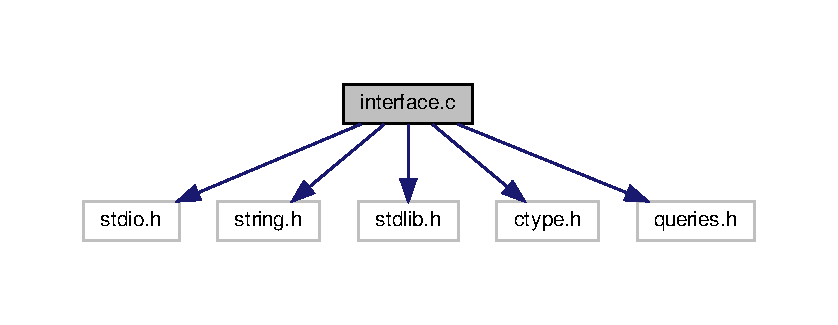
\includegraphics[width=350pt]{interface_8c__incl}
\end{center}
\end{figure}
\subsection*{Macros}
\begin{DoxyCompactItemize}
\item 
\mbox{\Hypertarget{interface_8c_acfe3a96b0125c2f51f936a9029ec6d18}\label{interface_8c_acfe3a96b0125c2f51f936a9029ec6d18}} 
\#define {\bfseries L\+T\+AM}~30
\end{DoxyCompactItemize}
\subsection*{Functions}
\begin{DoxyCompactItemize}
\item 
\mbox{\Hypertarget{interface_8c_adac116554b543b7c4228c018a85882f5}\label{interface_8c_adac116554b543b7c4228c018a85882f5}} 
void {\bfseries flush} ()
\item 
\mbox{\Hypertarget{interface_8c_a9e0170c5855c33f6721b8028b2e7947c}\label{interface_8c_a9e0170c5855c33f6721b8028b2e7947c}} 
int {\bfseries menudelistagem} (int j, int limit)
\item 
\mbox{\Hypertarget{interface_8c_aa031c499b7b3ef4f30cf24a5ff3934fe}\label{interface_8c_aa031c499b7b3ef4f30cf24a5ff3934fe}} 
void {\bfseries espacosparalistagem} (int i)
\item 
\mbox{\Hypertarget{interface_8c_aa2e2e035a2e067dd36ac276efc4fc8c7}\label{interface_8c_aa2e2e035a2e067dd36ac276efc4fc8c7}} 
void {\bfseries q2header} (char c, int i)
\item 
\mbox{\Hypertarget{interface_8c_a29b42d641636ea79c69c0ef737ad2a52}\label{interface_8c_a29b42d641636ea79c69c0ef737ad2a52}} 
void {\bfseries imprime\+Q2} (Q245 q, char op)
\item 
\mbox{\Hypertarget{interface_8c_a055b72ee6b865e6252eb88c936d3d773}\label{interface_8c_a055b72ee6b865e6252eb88c936d3d773}} 
void {\bfseries imprime\+Q3} (Q3 q, int \hyperlink{structmes}{mes}, int op)
\item 
\mbox{\Hypertarget{interface_8c_afbd904e15ece07140a1c980ef5eb832d}\label{interface_8c_afbd904e15ece07140a1c980ef5eb832d}} 
void {\bfseries q4header} (int f, int t)
\item 
\mbox{\Hypertarget{interface_8c_ab843072d51bc5c669ebf5e66b6d6c0a8}\label{interface_8c_ab843072d51bc5c669ebf5e66b6d6c0a8}} 
void {\bfseries imprime\+Q4} (Q245 q, int f)
\item 
\mbox{\Hypertarget{interface_8c_aec150235316abc233dd61a407bd302f5}\label{interface_8c_aec150235316abc233dd61a407bd302f5}} 
void {\bfseries q5header} (int t)
\item 
\mbox{\Hypertarget{interface_8c_a68bc092b53b60eed08cba9aa1e9386aa}\label{interface_8c_a68bc092b53b60eed08cba9aa1e9386aa}} 
void {\bfseries imprime\+Q5} (Q245 q)
\item 
\mbox{\Hypertarget{interface_8c_a34d4d5f87348ebc4fcd083ae524c9e40}\label{interface_8c_a34d4d5f87348ebc4fcd083ae524c9e40}} 
void {\bfseries imprime\+Q6} (Q6 q)
\item 
\mbox{\Hypertarget{interface_8c_a5a9badde6914191e0b9aa78a56bb281a}\label{interface_8c_a5a9badde6914191e0b9aa78a56bb281a}} 
void {\bfseries imprime\+Q7} (Q7 q)
\item 
\mbox{\Hypertarget{interface_8c_a0586df2ab2c24b95e88cb6e69f2cbc67}\label{interface_8c_a0586df2ab2c24b95e88cb6e69f2cbc67}} 
void {\bfseries imprime\+Q8} (Q8 q, int us, int op)
\item 
\mbox{\Hypertarget{interface_8c_aa6f894316d703f1127b1609ad96438b3}\label{interface_8c_aa6f894316d703f1127b1609ad96438b3}} 
void {\bfseries imprime\+Q9} (Q9 q, int \hyperlink{structfil}{fil})
\item 
\mbox{\Hypertarget{interface_8c_a8fc2725d7a23c82aa41d1632a369ad88}\label{interface_8c_a8fc2725d7a23c82aa41d1632a369ad88}} 
void {\bfseries imprime\+Q10} (Q12 q, int \hyperlink{structmes}{mes})
\item 
\mbox{\Hypertarget{interface_8c_a8774fa8b0f93a07211d336b50e19212d}\label{interface_8c_a8774fa8b0f93a07211d336b50e19212d}} 
void {\bfseries q11header} ()
\item 
\mbox{\Hypertarget{interface_8c_a416ff139c64f12959d2b47ee42a88ffe}\label{interface_8c_a416ff139c64f12959d2b47ee42a88ffe}} 
void {\bfseries imprime\+Q11} (Q11 q, int limit)
\item 
\mbox{\Hypertarget{interface_8c_a70e0725ea97a3572af73efa729ca8d89}\label{interface_8c_a70e0725ea97a3572af73efa729ca8d89}} 
void {\bfseries q12header} (int l, int t)
\item 
\mbox{\Hypertarget{interface_8c_ad10b16b7c692438e098a54e1874e54f0}\label{interface_8c_ad10b16b7c692438e098a54e1874e54f0}} 
void {\bfseries imprime\+Q12} (Q12 q, int limit)
\item 
\mbox{\Hypertarget{interface_8c_a4fb56cfc26efc42ca333df2ce9c0bc51}\label{interface_8c_a4fb56cfc26efc42ca333df2ce9c0bc51}} 
void {\bfseries imprime\+Q13} (Q13 q)
\item 
\mbox{\Hypertarget{interface_8c_aa21d4f60857a96693ccd5cfe2be8ddc1}\label{interface_8c_aa21d4f60857a96693ccd5cfe2be8ddc1}} 
void {\bfseries prettyprintmenu} ()
\item 
\mbox{\Hypertarget{interface_8c_a75d4023a2b14e7412fbf171d030e1f9c}\label{interface_8c_a75d4023a2b14e7412fbf171d030e1f9c}} 
int {\bfseries alldigits} (char $\ast$buf)
\item 
\mbox{\Hypertarget{interface_8c_a73ea7caddf8e661e9c85aebea9395d65}\label{interface_8c_a73ea7caddf8e661e9c85aebea9395d65}} 
int {\bfseries toint} (char $\ast$buf)
\item 
\mbox{\Hypertarget{interface_8c_a2182cfbcdb89e298c527ece9a5cff02f}\label{interface_8c_a2182cfbcdb89e298c527ece9a5cff02f}} 
void {\bfseries getstr} (char $\ast$text, char $\ast$s)
\item 
\mbox{\Hypertarget{interface_8c_a0785f1da9f5834c1f867a206ba7cbe8c}\label{interface_8c_a0785f1da9f5834c1f867a206ba7cbe8c}} 
void {\bfseries getint} (char $\ast$text, int $\ast$i)
\item 
\mbox{\Hypertarget{interface_8c_abdca1ef79a0ab12b7ed8575696e5c74d}\label{interface_8c_abdca1ef79a0ab12b7ed8575696e5c74d}} 
void {\bfseries interpertador} ()
\end{DoxyCompactItemize}


\subsection{Detailed Description}
Modulo que contém as funcções para apresentação das respostas as queries. 


\hypertarget{main_8c}{}\section{main.\+c File Reference}
\label{main_8c}\index{main.\+c@{main.\+c}}


Modulo main.  


{\ttfamily \#include \char`\"{}interface.\+h\char`\"{}}\newline
Include dependency graph for main.\+c\+:
\nopagebreak
\begin{figure}[H]
\begin{center}
\leavevmode
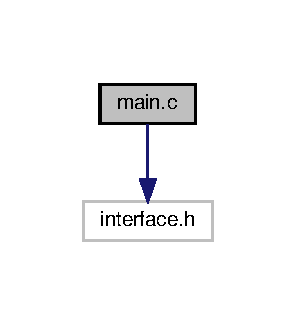
\includegraphics[width=142pt]{main_8c__incl}
\end{center}
\end{figure}
\subsection*{Functions}
\begin{DoxyCompactItemize}
\item 
\mbox{\Hypertarget{main_8c_ae66f6b31b5ad750f1fe042a706a4e3d4}\label{main_8c_ae66f6b31b5ad750f1fe042a706a4e3d4}} 
int {\bfseries main} ()
\end{DoxyCompactItemize}


\subsection{Detailed Description}
Modulo main. 


\hypertarget{produtos_8c}{}\section{produtos.\+c File Reference}
\label{produtos_8c}\index{produtos.\+c@{produtos.\+c}}


Modulo que contém as funções para leitura e validação de produtos.  


{\ttfamily \#include $<$stdio.\+h$>$}\newline
{\ttfamily \#include $<$string.\+h$>$}\newline
{\ttfamily \#include $<$stdlib.\+h$>$}\newline
{\ttfamily \#include \char`\"{}produtos.\+h\char`\"{}}\newline
Include dependency graph for produtos.\+c\+:
\nopagebreak
\begin{figure}[H]
\begin{center}
\leavevmode
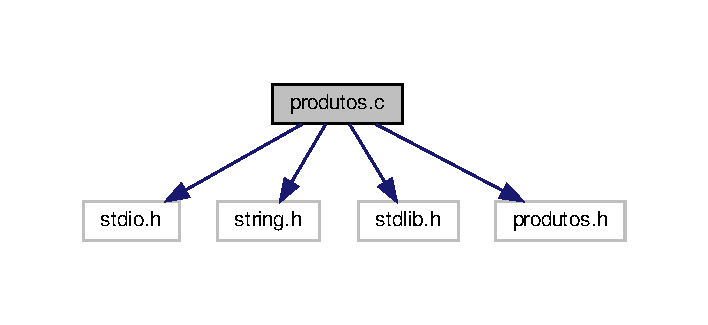
\includegraphics[width=340pt]{produtos_8c__incl}
\end{center}
\end{figure}
\subsection*{Classes}
\begin{DoxyCompactItemize}
\item 
struct \hyperlink{structbucket}{bucket}
\item 
struct \hyperlink{structthash}{thash}
\end{DoxyCompactItemize}
\subsection*{Typedefs}
\begin{DoxyCompactItemize}
\item 
\mbox{\Hypertarget{produtos_8c_ab73320ba1511b228e2d4df6fa47e8f1d}\label{produtos_8c_ab73320ba1511b228e2d4df6fa47e8f1d}} 
typedef struct \hyperlink{structbucket}{bucket} {\bfseries Bucket}
\item 
\mbox{\Hypertarget{produtos_8c_a21f0028bc00faa3267e3e3cc9ff2e271}\label{produtos_8c_a21f0028bc00faa3267e3e3cc9ff2e271}} 
typedef struct \hyperlink{structthash}{thash} {\bfseries T\+Hash}
\end{DoxyCompactItemize}
\subsection*{Functions}
\begin{DoxyCompactItemize}
\item 
int \hyperlink{produtos_8c_ad66fd4fdcccce5459a6beabc861284d4}{hash\+\_\+p} (char $\ast$cont)
\begin{DoxyCompactList}\small\item\em Função que recebe uma string e subtrai ao primeiro elemnto da string a letra A. \end{DoxyCompactList}\item 
\hyperlink{structthash}{T\+Hash} $\ast$ \hyperlink{produtos_8c_a421e774c98a70e1066cb43de34c81ccd}{init\+Tab\+\_\+p} ()
\begin{DoxyCompactList}\small\item\em Função que inicia uma estrutura Thash alocando espaço para todas as estruturas adjacentes. \end{DoxyCompactList}\item 
void \hyperlink{produtos_8c_a2455e1079c9d01e322fafeaa0cd985b0}{destroi\+Tab\+\_\+p} (\hyperlink{structthash}{T\+Hash} $\ast$h)
\begin{DoxyCompactList}\small\item\em Funçao que destroi uma estrutura Thash libertando o espaço ocupado por esta. \end{DoxyCompactList}\item 
void \hyperlink{produtos_8c_aff4e3384df1ecfdc932b0aab191e4783}{acrecensta\+Tab\+\_\+p} (\hyperlink{structthash}{T\+Hash} $\ast$h, char $\ast$cont)
\begin{DoxyCompactList}\small\item\em Função que acrescenta a uma Thash uma derminada string. \end{DoxyCompactList}\item 
void \hyperlink{produtos_8c_a05403823bd725ddc03baac6546a4f850}{swapp} (char $\ast$$\ast$arg1, char $\ast$$\ast$arg2)
\begin{DoxyCompactList}\small\item\em Função que troca duas strings de posicao. \end{DoxyCompactList}\item 
void \hyperlink{produtos_8c_a9d3a14dce1eae0512b438727b2b4e3ad}{quicksortp} (char $\ast$$\ast$args, unsigned int len)
\begin{DoxyCompactList}\small\item\em Função que ordena um array de strings. \end{DoxyCompactList}\item 
int \hyperlink{produtos_8c_aa361bd16a6960af3679506b2ab28d73f}{validaproduto} (char $\ast$produto)
\begin{DoxyCompactList}\small\item\em Função que recebe uma string de um produto e verifica se este é valido. \end{DoxyCompactList}\item 
int \hyperlink{produtos_8c_a188efbf6f79d9ac8f387745d3f1acdce}{ler\+\_\+prod} (\hyperlink{structthash}{T\+Hash} $\ast$prod, char $\ast$filespath, int $\ast$p)
\begin{DoxyCompactList}\small\item\em Função que le de um ficheiro para uma Thash. \end{DoxyCompactList}\item 
char $\ast$ \hyperlink{produtos_8c_ad4f27d1e9912da24cab63fb11aba8329}{get\+Produto} (\hyperlink{structthash}{T\+Hash} $\ast$p, int key, int i)
\begin{DoxyCompactList}\small\item\em Função que cria um clone de uma string produto. \end{DoxyCompactList}\item 
char $\ast$$\ast$ \hyperlink{produtos_8c_ad6e70ec8c69427882e8722e7cdbc5ffe}{get\+Array\+Prod} (\hyperlink{structthash}{T\+Hash} $\ast$p, int key)
\begin{DoxyCompactList}\small\item\em Função que cria um clone de um array de strings produto. \end{DoxyCompactList}\item 
int \hyperlink{produtos_8c_a08d1a3a77240188a65823a1173b2f361}{get\+Array\+Prod\+Size} (\hyperlink{structthash}{T\+Hash} $\ast$p, int key)
\begin{DoxyCompactList}\small\item\em Função que retorna o size um determinado array na tabela. \end{DoxyCompactList}\end{DoxyCompactItemize}


\subsection{Detailed Description}
Modulo que contém as funções para leitura e validação de produtos. 



\subsection{Function Documentation}
\mbox{\Hypertarget{produtos_8c_aff4e3384df1ecfdc932b0aab191e4783}\label{produtos_8c_aff4e3384df1ecfdc932b0aab191e4783}} 
\index{produtos.\+c@{produtos.\+c}!acrecensta\+Tab\+\_\+p@{acrecensta\+Tab\+\_\+p}}
\index{acrecensta\+Tab\+\_\+p@{acrecensta\+Tab\+\_\+p}!produtos.\+c@{produtos.\+c}}
\subsubsection{\texorpdfstring{acrecensta\+Tab\+\_\+p()}{acrecenstaTab\_p()}}
{\footnotesize\ttfamily void acrecensta\+Tab\+\_\+p (\begin{DoxyParamCaption}\item[{\hyperlink{structthash}{T\+Hash} $\ast$}]{h,  }\item[{char $\ast$}]{cont }\end{DoxyParamCaption})}



Função que acrescenta a uma Thash uma derminada string. 

Aplicando a função hash descobre a posicao correta desta na T\+Hash e sucessivamente realocando espaço para a adicionar á mesma


\begin{DoxyParams}{Parameters}
{\em T\+Hash} & $\ast$h T\+Hash previamente inicializada \\
\hline
{\em char} & $\ast$cont String genérica \\
\hline
\end{DoxyParams}
\mbox{\Hypertarget{produtos_8c_a2455e1079c9d01e322fafeaa0cd985b0}\label{produtos_8c_a2455e1079c9d01e322fafeaa0cd985b0}} 
\index{produtos.\+c@{produtos.\+c}!destroi\+Tab\+\_\+p@{destroi\+Tab\+\_\+p}}
\index{destroi\+Tab\+\_\+p@{destroi\+Tab\+\_\+p}!produtos.\+c@{produtos.\+c}}
\subsubsection{\texorpdfstring{destroi\+Tab\+\_\+p()}{destroiTab\_p()}}
{\footnotesize\ttfamily void destroi\+Tab\+\_\+p (\begin{DoxyParamCaption}\item[{\hyperlink{structthash}{T\+Hash} $\ast$}]{h }\end{DoxyParamCaption})}



Funçao que destroi uma estrutura Thash libertando o espaço ocupado por esta. 


\begin{DoxyParams}{Parameters}
{\em T\+Hash} & $\ast$h T\+Hash previamente inicializada \\
\hline
\end{DoxyParams}
\mbox{\Hypertarget{produtos_8c_ad6e70ec8c69427882e8722e7cdbc5ffe}\label{produtos_8c_ad6e70ec8c69427882e8722e7cdbc5ffe}} 
\index{produtos.\+c@{produtos.\+c}!get\+Array\+Prod@{get\+Array\+Prod}}
\index{get\+Array\+Prod@{get\+Array\+Prod}!produtos.\+c@{produtos.\+c}}
\subsubsection{\texorpdfstring{get\+Array\+Prod()}{getArrayProd()}}
{\footnotesize\ttfamily char$\ast$$\ast$ get\+Array\+Prod (\begin{DoxyParamCaption}\item[{\hyperlink{structthash}{T\+Hash} $\ast$}]{p,  }\item[{int}]{key }\end{DoxyParamCaption})}



Função que cria um clone de um array de strings produto. 


\begin{DoxyParams}{Parameters}
{\em T\+Hash} & $\ast$c Tabela de onde é retirado o produto \\
\hline
{\em int} & key indice na tabela\\
\hline
\end{DoxyParams}
\begin{DoxyReturn}{Returns}
char$\ast$$\ast$ Retorno da copia 
\end{DoxyReturn}
\mbox{\Hypertarget{produtos_8c_a08d1a3a77240188a65823a1173b2f361}\label{produtos_8c_a08d1a3a77240188a65823a1173b2f361}} 
\index{produtos.\+c@{produtos.\+c}!get\+Array\+Prod\+Size@{get\+Array\+Prod\+Size}}
\index{get\+Array\+Prod\+Size@{get\+Array\+Prod\+Size}!produtos.\+c@{produtos.\+c}}
\subsubsection{\texorpdfstring{get\+Array\+Prod\+Size()}{getArrayProdSize()}}
{\footnotesize\ttfamily int get\+Array\+Prod\+Size (\begin{DoxyParamCaption}\item[{\hyperlink{structthash}{T\+Hash} $\ast$}]{p,  }\item[{int}]{key }\end{DoxyParamCaption})}



Função que retorna o size um determinado array na tabela. 


\begin{DoxyParams}{Parameters}
{\em T\+Hash} & $\ast$c Tabela de onde é retirado o produto \\
\hline
{\em int} & key indice na tabela\\
\hline
\end{DoxyParams}
\begin{DoxyReturn}{Returns}
int Retorno do size 
\end{DoxyReturn}
\mbox{\Hypertarget{produtos_8c_ad4f27d1e9912da24cab63fb11aba8329}\label{produtos_8c_ad4f27d1e9912da24cab63fb11aba8329}} 
\index{produtos.\+c@{produtos.\+c}!get\+Produto@{get\+Produto}}
\index{get\+Produto@{get\+Produto}!produtos.\+c@{produtos.\+c}}
\subsubsection{\texorpdfstring{get\+Produto()}{getProduto()}}
{\footnotesize\ttfamily char$\ast$ get\+Produto (\begin{DoxyParamCaption}\item[{\hyperlink{structthash}{T\+Hash} $\ast$}]{p,  }\item[{int}]{key,  }\item[{int}]{i }\end{DoxyParamCaption})}



Função que cria um clone de uma string produto. 


\begin{DoxyParams}{Parameters}
{\em T\+Hash} & $\ast$c Tabela de onde é retirado o produto \\
\hline
{\em int} & key indice na tabela \\
\hline
{\em int} & i indice no array\\
\hline
\end{DoxyParams}
\begin{DoxyReturn}{Returns}
char$\ast$ Retorno da copia 
\end{DoxyReturn}
\mbox{\Hypertarget{produtos_8c_ad66fd4fdcccce5459a6beabc861284d4}\label{produtos_8c_ad66fd4fdcccce5459a6beabc861284d4}} 
\index{produtos.\+c@{produtos.\+c}!hash\+\_\+p@{hash\+\_\+p}}
\index{hash\+\_\+p@{hash\+\_\+p}!produtos.\+c@{produtos.\+c}}
\subsubsection{\texorpdfstring{hash\+\_\+p()}{hash\_p()}}
{\footnotesize\ttfamily int hash\+\_\+p (\begin{DoxyParamCaption}\item[{char $\ast$}]{cont }\end{DoxyParamCaption})}



Função que recebe uma string e subtrai ao primeiro elemnto da string a letra A. 


\begin{DoxyParams}{Parameters}
{\em char} & $\ast$cont String genérica\\
\hline
\end{DoxyParams}
\begin{DoxyReturn}{Returns}
int O resultado inteiro dessa subtração 
\end{DoxyReturn}
\mbox{\Hypertarget{produtos_8c_a421e774c98a70e1066cb43de34c81ccd}\label{produtos_8c_a421e774c98a70e1066cb43de34c81ccd}} 
\index{produtos.\+c@{produtos.\+c}!init\+Tab\+\_\+p@{init\+Tab\+\_\+p}}
\index{init\+Tab\+\_\+p@{init\+Tab\+\_\+p}!produtos.\+c@{produtos.\+c}}
\subsubsection{\texorpdfstring{init\+Tab\+\_\+p()}{initTab\_p()}}
{\footnotesize\ttfamily \hyperlink{structthash}{T\+Hash}$\ast$ init\+Tab\+\_\+p (\begin{DoxyParamCaption}{ }\end{DoxyParamCaption})}



Função que inicia uma estrutura Thash alocando espaço para todas as estruturas adjacentes. 

\begin{DoxyReturn}{Returns}
T\+Hash$\ast$ Devolve a T\+Hash inicializada 
\end{DoxyReturn}
\mbox{\Hypertarget{produtos_8c_a188efbf6f79d9ac8f387745d3f1acdce}\label{produtos_8c_a188efbf6f79d9ac8f387745d3f1acdce}} 
\index{produtos.\+c@{produtos.\+c}!ler\+\_\+prod@{ler\+\_\+prod}}
\index{ler\+\_\+prod@{ler\+\_\+prod}!produtos.\+c@{produtos.\+c}}
\subsubsection{\texorpdfstring{ler\+\_\+prod()}{ler\_prod()}}
{\footnotesize\ttfamily int ler\+\_\+prod (\begin{DoxyParamCaption}\item[{\hyperlink{structthash}{T\+Hash} $\ast$}]{prod,  }\item[{char $\ast$}]{filespath,  }\item[{int $\ast$}]{p }\end{DoxyParamCaption})}



Função que le de um ficheiro para uma Thash. 

Recebendo uma Thash e um file path, lê de um ficheiro linha a linha e vai colocando cada linha na thash na sua posição correspondente na mesma


\begin{DoxyParams}{Parameters}
{\em T\+Hash} & $\ast$prod T\+Hash onde vai ser colocada a informação \\
\hline
{\em char} & $\ast$filespath String com o file path \\
\hline
{\em int} & $\ast$p Inteiro onde é guardado o numero de produtos lidos\\
\hline
\end{DoxyParams}
\begin{DoxyReturn}{Returns}
int O numero de produtos válidos 
\end{DoxyReturn}
\mbox{\Hypertarget{produtos_8c_a9d3a14dce1eae0512b438727b2b4e3ad}\label{produtos_8c_a9d3a14dce1eae0512b438727b2b4e3ad}} 
\index{produtos.\+c@{produtos.\+c}!quicksortp@{quicksortp}}
\index{quicksortp@{quicksortp}!produtos.\+c@{produtos.\+c}}
\subsubsection{\texorpdfstring{quicksortp()}{quicksortp()}}
{\footnotesize\ttfamily void quicksortp (\begin{DoxyParamCaption}\item[{char $\ast$$\ast$}]{args,  }\item[{unsigned int}]{len }\end{DoxyParamCaption})}



Função que ordena um array de strings. 


\begin{DoxyParams}{Parameters}
{\em unsigned} & int len int tam generico \\
\hline
{\em char} & $\ast$$\ast$args String genérica \\
\hline
\end{DoxyParams}
\mbox{\Hypertarget{produtos_8c_a05403823bd725ddc03baac6546a4f850}\label{produtos_8c_a05403823bd725ddc03baac6546a4f850}} 
\index{produtos.\+c@{produtos.\+c}!swapp@{swapp}}
\index{swapp@{swapp}!produtos.\+c@{produtos.\+c}}
\subsubsection{\texorpdfstring{swapp()}{swapp()}}
{\footnotesize\ttfamily void swapp (\begin{DoxyParamCaption}\item[{char $\ast$$\ast$}]{arg1,  }\item[{char $\ast$$\ast$}]{arg2 }\end{DoxyParamCaption})}



Função que troca duas strings de posicao. 


\begin{DoxyParams}{Parameters}
{\em char} & $\ast$$\ast$arg1 String genérica \\
\hline
{\em char} & $\ast$$\ast$arg2 String genérica \\
\hline
\end{DoxyParams}
\mbox{\Hypertarget{produtos_8c_aa361bd16a6960af3679506b2ab28d73f}\label{produtos_8c_aa361bd16a6960af3679506b2ab28d73f}} 
\index{produtos.\+c@{produtos.\+c}!validaproduto@{validaproduto}}
\index{validaproduto@{validaproduto}!produtos.\+c@{produtos.\+c}}
\subsubsection{\texorpdfstring{validaproduto()}{validaproduto()}}
{\footnotesize\ttfamily int validaproduto (\begin{DoxyParamCaption}\item[{char $\ast$}]{produto }\end{DoxyParamCaption})}



Função que recebe uma string de um produto e verifica se este é valido. 


\begin{DoxyParams}{Parameters}
{\em char} & $\ast$produto String (produto)\\
\hline
\end{DoxyParams}
\begin{DoxyReturn}{Returns}
int 
\end{DoxyReturn}

\hypertarget{queries_8c}{}\section{queries.\+c File Reference}
\label{queries_8c}\index{queries.\+c@{queries.\+c}}


Modulo que contém as funcções de resposta as queries.  


{\ttfamily \#include $<$stdio.\+h$>$}\newline
{\ttfamily \#include $<$string.\+h$>$}\newline
{\ttfamily \#include $<$stdlib.\+h$>$}\newline
{\ttfamily \#include \char`\"{}clientes.\+h\char`\"{}}\newline
{\ttfamily \#include \char`\"{}produtos.\+h\char`\"{}}\newline
{\ttfamily \#include \char`\"{}faturacao.\+h\char`\"{}}\newline
{\ttfamily \#include \char`\"{}filiais.\+h\char`\"{}}\newline
{\ttfamily \#include \char`\"{}vendas.\+h\char`\"{}}\newline
{\ttfamily \#include \char`\"{}queries.\+h\char`\"{}}\newline
Include dependency graph for queries.\+c\+:
\nopagebreak
\begin{figure}[H]
\begin{center}
\leavevmode
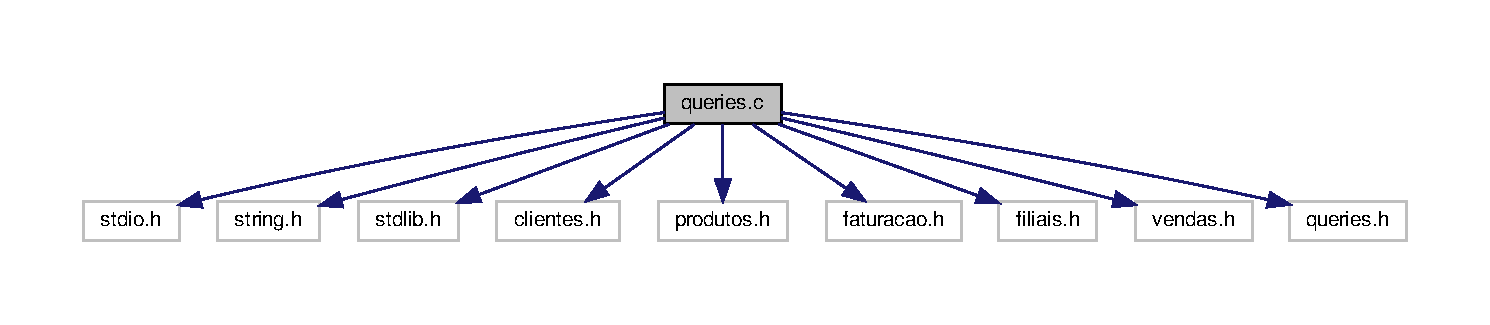
\includegraphics[width=350pt]{queries_8c__incl}
\end{center}
\end{figure}
\subsection*{Classes}
\begin{DoxyCompactItemize}
\item 
struct \hyperlink{structsgv}{sgv}
\end{DoxyCompactItemize}
\subsection*{Typedefs}
\begin{DoxyCompactItemize}
\item 
\mbox{\Hypertarget{queries_8c_a353ab4b59e69f777538389a7d3d90a74}\label{queries_8c_a353ab4b59e69f777538389a7d3d90a74}} 
typedef struct \hyperlink{structsgv}{sgv} $\ast$ {\bfseries S\+GV}
\end{DoxyCompactItemize}
\subsection*{Functions}
\begin{DoxyCompactItemize}
\item 
\mbox{\Hypertarget{queries_8c_a14c3840c38c574667ca887b40c5250bb}\label{queries_8c_a14c3840c38c574667ca887b40c5250bb}} 
\hyperlink{structsgv}{S\+GV} {\bfseries init\+S\+GV} ()
\item 
\mbox{\Hypertarget{queries_8c_aea434f0f0491f9325976a85e46447a5c}\label{queries_8c_aea434f0f0491f9325976a85e46447a5c}} 
void {\bfseries distroy\+S\+GV} (\hyperlink{structsgv}{S\+GV} \hyperlink{structsgv}{sgv})
\item 
\mbox{\Hypertarget{queries_8c_a4da6b42210fa75c7b69ed3991b4ed669}\label{queries_8c_a4da6b42210fa75c7b69ed3991b4ed669}} 
void {\bfseries destroi\+Array\+Strings} (char $\ast$$\ast$a, int size)
\item 
int \hyperlink{queries_8c_af837160764e31ee7884fd175306e88ba}{validames} (int m)
\begin{DoxyCompactList}\small\item\em Função que verifica se um mes é valido testando se o int dado está entre 0 e 12. \end{DoxyCompactList}\item 
int \hyperlink{queries_8c_a43f0d44bfa5f2e6f5ed4086a53bea448}{validafilial} (int f)
\begin{DoxyCompactList}\small\item\em Função que verifica se uma filial é valida testando se o int dado está entre 1 e 3. \end{DoxyCompactList}\item 
\mbox{\Hypertarget{queries_8c_a9699793c6090e44f1908416d02a7aa2a}\label{queries_8c_a9699793c6090e44f1908416d02a7aa2a}} 
int {\bfseries letravalida} (char l)
\item 
\mbox{\Hypertarget{queries_8c_a0e5d092c192d7f1643bf2a93e564e4a5}\label{queries_8c_a0e5d092c192d7f1643bf2a93e564e4a5}} 
\hyperlink{structsgv}{S\+GV} {\bfseries load\+S\+G\+V\+From\+Files} (\hyperlink{structsgv}{S\+GV} \hyperlink{structsgv}{sgv}, char $\ast$clients\+File\+Path, char $\ast$products\+File\+Path, char $\ast$sales\+File\+Path)
\item 
\mbox{\Hypertarget{queries_8c_add4049af28831b953f9046a771964e92}\label{queries_8c_add4049af28831b953f9046a771964e92}} 
Q245 {\bfseries get\+Products\+Started\+By\+Letter} (\hyperlink{structsgv}{S\+GV} \hyperlink{structsgv}{sgv}, char letter)
\item 
\mbox{\Hypertarget{queries_8c_a467a12d16e3ae3b0b5be3d01ebd1a085}\label{queries_8c_a467a12d16e3ae3b0b5be3d01ebd1a085}} 
void {\bfseries destroi\+Q245} (Q245 q)
\item 
\mbox{\Hypertarget{queries_8c_ace24a94642a885c9468602cd0d9f9db4}\label{queries_8c_ace24a94642a885c9468602cd0d9f9db4}} 
Q3 {\bfseries get\+Products\+Sales\+And\+Profit} (\hyperlink{structsgv}{S\+GV} \hyperlink{structsgv}{sgv}, char $\ast$product\+ID, int month)
\item 
\mbox{\Hypertarget{queries_8c_a1e3c207ad0a048b23e3487622148935f}\label{queries_8c_a1e3c207ad0a048b23e3487622148935f}} 
void {\bfseries destroi\+Q3} (Q3 q)
\item 
\mbox{\Hypertarget{queries_8c_aeacadbc70071c706bfbf8769dc799cc0}\label{queries_8c_aeacadbc70071c706bfbf8769dc799cc0}} 
Q245 {\bfseries get\+Products\+Never\+Bought} (\hyperlink{structsgv}{S\+GV} \hyperlink{structsgv}{sgv}, int branch\+ID)
\item 
\mbox{\Hypertarget{queries_8c_adc2fedfb59b20693db3b55df0fcb7472}\label{queries_8c_adc2fedfb59b20693db3b55df0fcb7472}} 
Q245 {\bfseries get\+Clients\+Of\+All\+Branches} (\hyperlink{structsgv}{S\+GV} \hyperlink{structsgv}{sgv})
\item 
\mbox{\Hypertarget{queries_8c_a2a4624f046ebc2609ce4fa1697c832da}\label{queries_8c_a2a4624f046ebc2609ce4fa1697c832da}} 
Q6 {\bfseries get\+Clients\+And\+Products\+Never\+Bought\+Count} (\hyperlink{structsgv}{S\+GV} \hyperlink{structsgv}{sgv})
\item 
\mbox{\Hypertarget{queries_8c_ab6a4cba5785b2803cb1d80e0d0c8fdc7}\label{queries_8c_ab6a4cba5785b2803cb1d80e0d0c8fdc7}} 
void {\bfseries destroi\+Q6} (Q6 q)
\item 
\mbox{\Hypertarget{queries_8c_a44987d4ab3920bd87edcf2b26dacabb4}\label{queries_8c_a44987d4ab3920bd87edcf2b26dacabb4}} 
Q7 {\bfseries get\+Products\+Bought\+By\+Client} (\hyperlink{structsgv}{S\+GV} \hyperlink{structsgv}{sgv}, char $\ast$client\+ID)
\item 
\mbox{\Hypertarget{queries_8c_a9a1b1562ba4f92a40566b6ba8cb32c31}\label{queries_8c_a9a1b1562ba4f92a40566b6ba8cb32c31}} 
void {\bfseries destroi\+Q7} (Q7 q)
\item 
\mbox{\Hypertarget{queries_8c_ab2beb2db827fb78a405ccb58405f9fb7}\label{queries_8c_ab2beb2db827fb78a405ccb58405f9fb7}} 
Q8 {\bfseries get\+Sales\+And\+Profif} (\hyperlink{structsgv}{S\+GV} \hyperlink{structsgv}{sgv}, int min\+Month, int max\+Month)
\item 
\mbox{\Hypertarget{queries_8c_aa8d0a586a0ea7c137ccd32c0ed8ee7fa}\label{queries_8c_aa8d0a586a0ea7c137ccd32c0ed8ee7fa}} 
void {\bfseries destroi\+Q8} (Q8 q)
\item 
\mbox{\Hypertarget{queries_8c_a64de436cdf84b48f05143ab00ab4988f}\label{queries_8c_a64de436cdf84b48f05143ab00ab4988f}} 
Q9 {\bfseries get\+Product\+Buyers} (\hyperlink{structsgv}{S\+GV} \hyperlink{structsgv}{sgv}, char $\ast$product\+ID, int branch)
\item 
\mbox{\Hypertarget{queries_8c_a0ed9e1eb48f33025118e482fad051647}\label{queries_8c_a0ed9e1eb48f33025118e482fad051647}} 
void {\bfseries destroi\+Q9} (Q9 q)
\item 
void \hyperlink{queries_8c_a5e077712c251785d4e50e9a96e460f22}{swapq12} (Qnt\+N\+Spent $\ast$args, int i1, int i2)
\begin{DoxyCompactList}\small\item\em Função que troca duas estruturas Qnt\+Spent de posicao num array. \end{DoxyCompactList}\item 
void \hyperlink{queries_8c_a54d6022abb41c2c5fd93742ac2e24168}{q10sort} (Qnt\+N\+Spent $\ast$args, int len)
\begin{DoxyCompactList}\small\item\em Função que ordena um array de estruturas Qnt\+Spent. \end{DoxyCompactList}\item 
\mbox{\Hypertarget{queries_8c_aab4db29061bfb157fd70e93276f27cba}\label{queries_8c_aab4db29061bfb157fd70e93276f27cba}} 
Q12 {\bfseries get\+Client\+Favourite\+Products} (\hyperlink{structsgv}{S\+GV} \hyperlink{structsgv}{sgv}, char $\ast$client\+ID, int month)
\item 
\mbox{\Hypertarget{queries_8c_a2b39aa0e8c1e3d00663eed8895c16e38}\label{queries_8c_a2b39aa0e8c1e3d00663eed8895c16e38}} 
void {\bfseries destroi\+Q12} (Q12 q)
\item 
\mbox{\Hypertarget{queries_8c_a974316c75d13c9b140f030b415f1d999}\label{queries_8c_a974316c75d13c9b140f030b415f1d999}} 
void {\bfseries swapq11} (Qt $\ast$args, int i1, int i2)
\item 
\mbox{\Hypertarget{queries_8c_a3f8fcf52b20f593e4671818081913762}\label{queries_8c_a3f8fcf52b20f593e4671818081913762}} 
void {\bfseries q11sort} (Qt $\ast$args, int len)
\item 
\mbox{\Hypertarget{queries_8c_a12540147c145027bbf9d1841db93bc60}\label{queries_8c_a12540147c145027bbf9d1841db93bc60}} 
Q11 {\bfseries init\+Q11} ()
\item 
\mbox{\Hypertarget{queries_8c_a9c6f8721ddae42220a860c98b94b7e09}\label{queries_8c_a9c6f8721ddae42220a860c98b94b7e09}} 
int {\bfseries existe\+Prod} (Qt $\ast$arr, char $\ast$procurado, int Tam)
\item 
\mbox{\Hypertarget{queries_8c_adf10a4dfa4f15639efa26fba7d22d409}\label{queries_8c_adf10a4dfa4f15639efa26fba7d22d409}} 
Q11 {\bfseries to\+Array} (\hyperlink{structsgv}{S\+GV} \hyperlink{structsgv}{sgv})
\item 
\mbox{\Hypertarget{queries_8c_af17ac312fe5912a174935b9b9f10d624}\label{queries_8c_af17ac312fe5912a174935b9b9f10d624}} 
void {\bfseries um\+Cliente} (\hyperlink{structsgv}{S\+GV} \hyperlink{structsgv}{sgv}, Q11 q, int k, int id)
\item 
\mbox{\Hypertarget{queries_8c_a0b8274230dfe854c8410d4f728a10206}\label{queries_8c_a0b8274230dfe854c8410d4f728a10206}} 
Q11 {\bfseries get\+Top\+Selled\+Products} (\hyperlink{structsgv}{S\+GV} \hyperlink{structsgv}{sgv}, int limit)
\item 
\mbox{\Hypertarget{queries_8c_a22823cdbbfd351c9aacb39937a2d9748}\label{queries_8c_a22823cdbbfd351c9aacb39937a2d9748}} 
void {\bfseries destroi\+Q11} (Q11 q)
\item 
\mbox{\Hypertarget{queries_8c_a9baba84818d94899ef0b11640c800f04}\label{queries_8c_a9baba84818d94899ef0b11640c800f04}} 
Q12 {\bfseries init\+Q12} ()
\item 
\mbox{\Hypertarget{queries_8c_ad57bbed4fd58195d60359e9bf219457d}\label{queries_8c_ad57bbed4fd58195d60359e9bf219457d}} 
void {\bfseries q12sort} (Qnt\+N\+Spent $\ast$args, int len)
\item 
\mbox{\Hypertarget{queries_8c_af277ed9df5b7cbfe2e83dd9a4b258f47}\label{queries_8c_af277ed9df5b7cbfe2e83dd9a4b258f47}} 
int {\bfseries existe\+\_\+q12} (Qnt\+N\+Spent $\ast$arr, char $\ast$procurado, int Tam)
\item 
\mbox{\Hypertarget{queries_8c_ade07fddcdb86a6494fb7fd0e13182f97}\label{queries_8c_ade07fddcdb86a6494fb7fd0e13182f97}} 
Q12 {\bfseries get\+Client\+Top\+Profit\+Products} (\hyperlink{structsgv}{S\+GV} \hyperlink{structsgv}{sgv}, char $\ast$client\+ID, int limit)
\item 
\mbox{\Hypertarget{queries_8c_ab3aed9406f5817f7a483ac0e083b6f1a}\label{queries_8c_ab3aed9406f5817f7a483ac0e083b6f1a}} 
char $\ast$ {\bfseries get\+Read\+File} (char $\ast$file\+Path)
\item 
\mbox{\Hypertarget{queries_8c_a5e8b275d70dd3b53c77c8bec2d476b3a}\label{queries_8c_a5e8b275d70dd3b53c77c8bec2d476b3a}} 
Q13 {\bfseries get\+Current\+Files\+Info} (\hyperlink{structsgv}{S\+GV} \hyperlink{structsgv}{sgv})
\item 
\mbox{\Hypertarget{queries_8c_aae2361dd6a47e31f23241b5530129de6}\label{queries_8c_aae2361dd6a47e31f23241b5530129de6}} 
void {\bfseries destroi\+Q13} (Q13 q)
\end{DoxyCompactItemize}


\subsection{Detailed Description}
Modulo que contém as funcções de resposta as queries. 



\subsection{Function Documentation}
\mbox{\Hypertarget{queries_8c_a54d6022abb41c2c5fd93742ac2e24168}\label{queries_8c_a54d6022abb41c2c5fd93742ac2e24168}} 
\index{queries.\+c@{queries.\+c}!q10sort@{q10sort}}
\index{q10sort@{q10sort}!queries.\+c@{queries.\+c}}
\subsubsection{\texorpdfstring{q10sort()}{q10sort()}}
{\footnotesize\ttfamily void q10sort (\begin{DoxyParamCaption}\item[{Qnt\+N\+Spent $\ast$}]{args,  }\item[{int}]{len }\end{DoxyParamCaption})}



Função que ordena um array de estruturas Qnt\+Spent. 


\begin{DoxyParams}{Parameters}
{\em Qnt\+Spent} & $\ast$args Array de Estruturas \\
\hline
{\em int} & len Comprimento do array \\
\hline
\end{DoxyParams}
\mbox{\Hypertarget{queries_8c_a5e077712c251785d4e50e9a96e460f22}\label{queries_8c_a5e077712c251785d4e50e9a96e460f22}} 
\index{queries.\+c@{queries.\+c}!swapq12@{swapq12}}
\index{swapq12@{swapq12}!queries.\+c@{queries.\+c}}
\subsubsection{\texorpdfstring{swapq12()}{swapq12()}}
{\footnotesize\ttfamily void swapq12 (\begin{DoxyParamCaption}\item[{Qnt\+N\+Spent $\ast$}]{args,  }\item[{int}]{i1,  }\item[{int}]{i2 }\end{DoxyParamCaption})}



Função que troca duas estruturas Qnt\+Spent de posicao num array. 


\begin{DoxyParams}{Parameters}
{\em Qnt\+Spent} & $\ast$args Array de Estruturas \\
\hline
{\em int} & i1 Indice no array da primeira estrutura \\
\hline
{\em int} & i2 Indice no array da segunda estrutura \\
\hline
\end{DoxyParams}
\mbox{\Hypertarget{queries_8c_a43f0d44bfa5f2e6f5ed4086a53bea448}\label{queries_8c_a43f0d44bfa5f2e6f5ed4086a53bea448}} 
\index{queries.\+c@{queries.\+c}!validafilial@{validafilial}}
\index{validafilial@{validafilial}!queries.\+c@{queries.\+c}}
\subsubsection{\texorpdfstring{validafilial()}{validafilial()}}
{\footnotesize\ttfamily int validafilial (\begin{DoxyParamCaption}\item[{int}]{f }\end{DoxyParamCaption})}



Função que verifica se uma filial é valida testando se o int dado está entre 1 e 3. 

caso sim dá retorno 1, caso contrário -\/1


\begin{DoxyParams}{Parameters}
{\em int} & f Filial a testar\\
\hline
\end{DoxyParams}
\begin{DoxyReturn}{Returns}
int 
\end{DoxyReturn}
\mbox{\Hypertarget{queries_8c_af837160764e31ee7884fd175306e88ba}\label{queries_8c_af837160764e31ee7884fd175306e88ba}} 
\index{queries.\+c@{queries.\+c}!validames@{validames}}
\index{validames@{validames}!queries.\+c@{queries.\+c}}
\subsubsection{\texorpdfstring{validames()}{validames()}}
{\footnotesize\ttfamily int validames (\begin{DoxyParamCaption}\item[{int}]{m }\end{DoxyParamCaption})}



Função que verifica se um mes é valido testando se o int dado está entre 0 e 12. 

caso sim dá retorno 1, caso contrário -\/1


\begin{DoxyParams}{Parameters}
{\em int} & m Mes a testar\\
\hline
\end{DoxyParams}
\begin{DoxyReturn}{Returns}
int 
\end{DoxyReturn}

\hypertarget{vendas_8c}{}\section{vendas.\+c File Reference}
\label{vendas_8c}\index{vendas.\+c@{vendas.\+c}}


Modulo que contém as funcções para leitura e validação de vendas e incorporação destas nas estruturas filiais e faturação.  


{\ttfamily \#include $<$stdio.\+h$>$}\newline
{\ttfamily \#include $<$string.\+h$>$}\newline
{\ttfamily \#include $<$stdlib.\+h$>$}\newline
{\ttfamily \#include $<$ctype.\+h$>$}\newline
{\ttfamily \#include \char`\"{}clientes.\+h\char`\"{}}\newline
{\ttfamily \#include \char`\"{}faturacao.\+h\char`\"{}}\newline
{\ttfamily \#include \char`\"{}filiais.\+h\char`\"{}}\newline
{\ttfamily \#include \char`\"{}produtos.\+h\char`\"{}}\newline
{\ttfamily \#include \char`\"{}vendas.\+h\char`\"{}}\newline
Include dependency graph for vendas.\+c\+:
\nopagebreak
\begin{figure}[H]
\begin{center}
\leavevmode
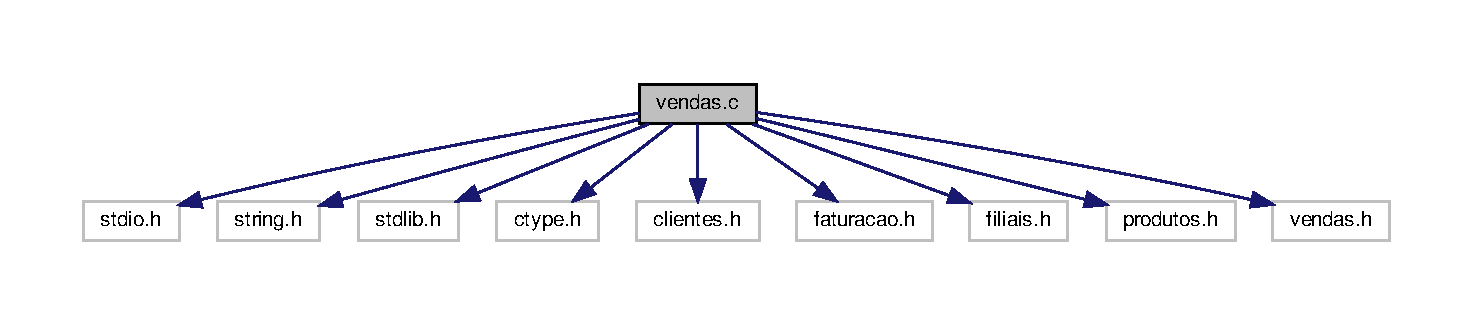
\includegraphics[width=350pt]{vendas_8c__incl}
\end{center}
\end{figure}
\subsection*{Functions}
\begin{DoxyCompactItemize}
\item 
\mbox{\Hypertarget{vendas_8c_a51f66e1e24f722303640d1da8824c0e8}\label{vendas_8c_a51f66e1e24f722303640d1da8824c0e8}} 
int {\bfseries alldigit} (char $\ast$buf)
\item 
\mbox{\Hypertarget{vendas_8c_ab7e033bbd635e77371051ef24749e89b}\label{vendas_8c_ab7e033bbd635e77371051ef24749e89b}} 
int {\bfseries isfloat} (char $\ast$campo)
\item 
void \hyperlink{vendas_8c_a71c6b46d6c27c5d05443e4f4680240db}{destroi\+Array\+String} (char $\ast$$\ast$a, int size)
\item 
int \hyperlink{vendas_8c_a17e5ea168e2a616942e52667f8285984}{existe} (char $\ast$$\ast$testado, char $\ast$nas\+\_\+vendas, int Tam)
\begin{DoxyCompactList}\small\item\em Função de procura binária, que procura num array de strings uma string. \end{DoxyCompactList}\item 
int \hyperlink{vendas_8c_aec6ea11d2c2ce802a6a0209b8743aaf7}{validapreco} (char $\ast$preco)
\begin{DoxyCompactList}\small\item\em Função que verifica se um preçe é valido testando se esse preço se encontra entre dois valores. \end{DoxyCompactList}\item 
int \hyperlink{vendas_8c_a38f966df1d4e99b7246228216620e155}{valida3campo} (char $\ast$campo)
\begin{DoxyCompactList}\small\item\em Função que verifica se uma quantidade é valida testando se esse valor se encontra entre dois valores. \end{DoxyCompactList}\item 
int \hyperlink{vendas_8c_a17cd0a6871ad958086895d8dc257ea6b}{valida4campo} (char $\ast$campo)
\begin{DoxyCompactList}\small\item\em Função que verifica se um tipo de compra é valido testando se o char dado é válido. \end{DoxyCompactList}\item 
int \hyperlink{vendas_8c_a27545cd0e98a95674365948cad34ec83}{valida6mes} (char $\ast$campo)
\begin{DoxyCompactList}\small\item\em Função que verifica se um mes é valido testando se o int dado está entre 0 e 12. \end{DoxyCompactList}\item 
int \hyperlink{vendas_8c_a565a8e4b425bac6d01b4ec4ec46d84e7}{valida7filial} (char $\ast$\hyperlink{structfilial}{filial})
\begin{DoxyCompactList}\small\item\em Função que verifica se uma filial é valida testando se o int dado está entre 1 e 3. \end{DoxyCompactList}\item 
int \hyperlink{vendas_8c_a9d66eb71dbdb558536023b991bc29bb6}{ler\+\_\+venda} (\hyperlink{structfat}{Fat} $\ast$\hyperlink{structfat}{fat}, \hyperlink{structfilial}{Filial} $\ast$\hyperlink{structfil}{fil}, \hyperlink{structthash}{T\+Hash} $\ast$cliente, \hyperlink{structthash}{T\+Hash} $\ast$prod, char $\ast$filespath, int $\ast$v)
\begin{DoxyCompactList}\small\item\em Função que le de um ficheiro Vendas. \end{DoxyCompactList}\end{DoxyCompactItemize}


\subsection{Detailed Description}
Modulo que contém as funcções para leitura e validação de vendas e incorporação destas nas estruturas filiais e faturação. 



\subsection{Function Documentation}
\mbox{\Hypertarget{vendas_8c_a71c6b46d6c27c5d05443e4f4680240db}\label{vendas_8c_a71c6b46d6c27c5d05443e4f4680240db}} 
\index{vendas.\+c@{vendas.\+c}!destroi\+Array\+String@{destroi\+Array\+String}}
\index{destroi\+Array\+String@{destroi\+Array\+String}!vendas.\+c@{vendas.\+c}}
\subsubsection{\texorpdfstring{destroi\+Array\+String()}{destroiArrayString()}}
{\footnotesize\ttfamily void destroi\+Array\+String (\begin{DoxyParamCaption}\item[{char $\ast$$\ast$}]{a,  }\item[{int}]{size }\end{DoxyParamCaption})}

Função que destroi (liberta) um array de strings 
\begin{DoxyParams}{Parameters}
{\em char} & $\ast$$\ast$a \\
\hline
{\em int} & size \\
\hline
\end{DoxyParams}
\mbox{\Hypertarget{vendas_8c_a17e5ea168e2a616942e52667f8285984}\label{vendas_8c_a17e5ea168e2a616942e52667f8285984}} 
\index{vendas.\+c@{vendas.\+c}!existe@{existe}}
\index{existe@{existe}!vendas.\+c@{vendas.\+c}}
\subsubsection{\texorpdfstring{existe()}{existe()}}
{\footnotesize\ttfamily int existe (\begin{DoxyParamCaption}\item[{char $\ast$$\ast$}]{testado,  }\item[{char $\ast$}]{nas\+\_\+vendas,  }\item[{int}]{Tam }\end{DoxyParamCaption})}



Função de procura binária, que procura num array de strings uma string. 

Quando a encontra retorna 1 , caso não encontre retorna 0


\begin{DoxyParams}{Parameters}
{\em char} & $\ast$$\ast$testado Array genérico \\
\hline
{\em char} & $\ast$nas\+\_\+vendas Uma string genérica \\
\hline
{\em int} & Tam Um int size\\
\hline
\end{DoxyParams}
\begin{DoxyReturn}{Returns}
int r O indice se encontrado 
\end{DoxyReturn}
\mbox{\Hypertarget{vendas_8c_a9d66eb71dbdb558536023b991bc29bb6}\label{vendas_8c_a9d66eb71dbdb558536023b991bc29bb6}} 
\index{vendas.\+c@{vendas.\+c}!ler\+\_\+venda@{ler\+\_\+venda}}
\index{ler\+\_\+venda@{ler\+\_\+venda}!vendas.\+c@{vendas.\+c}}
\subsubsection{\texorpdfstring{ler\+\_\+venda()}{ler\_venda()}}
{\footnotesize\ttfamily int ler\+\_\+venda (\begin{DoxyParamCaption}\item[{\hyperlink{structfat}{Fat} $\ast$}]{fat,  }\item[{\hyperlink{structfilial}{Filial} $\ast$}]{fil,  }\item[{\hyperlink{structthash}{T\+Hash} $\ast$}]{cliente,  }\item[{\hyperlink{structthash}{T\+Hash} $\ast$}]{prod,  }\item[{char $\ast$}]{filespath,  }\item[{int $\ast$}]{v }\end{DoxyParamCaption})}



Função que le de um ficheiro Vendas. 

Recebendo uma Fat (estrutura Faturação),uma Filial (estrutura Filial) e duas T\+Hash(estruturas clientes e produtos) e um file path, lê linha a linha de um determinado ficheiro fazendo enquanto este válido a divisão por espaços  e ~\newline
, vai repassando as partes retiradas dessa linha para uma string part, que vai sendo guardada em auxiliares-\/ Postriormente os campos retirados da linha são validados e são alocados pelas funcçoes acrescenta\+Fat e acrescenta\+Fil as respetivas estruturas que estas recebem como argumento;


\begin{DoxyParams}{Parameters}
{\em Fat} & $\ast$fat Estrutura Fat para onde vai ser extraida informação do ficheiro \\
\hline
{\em Filial} & $\ast$fil Estrutura Filial para onde vai ser extraida informação do ficheiro \\
\hline
{\em T\+Hash} & $\ast$cliente Estrutura T\+Hash para onde vai ser extraida informação do ficheiro \\
\hline
{\em char} & $\ast$filespath File path do ficheiro a ler \\
\hline
{\em int} & $\ast$v $\ast$int onde se vai guardar o total de vendas lidas\\
\hline
\end{DoxyParams}
\begin{DoxyReturn}{Returns}
int int numero de vendas válidas 
\end{DoxyReturn}
\mbox{\Hypertarget{vendas_8c_a38f966df1d4e99b7246228216620e155}\label{vendas_8c_a38f966df1d4e99b7246228216620e155}} 
\index{vendas.\+c@{vendas.\+c}!valida3campo@{valida3campo}}
\index{valida3campo@{valida3campo}!vendas.\+c@{vendas.\+c}}
\subsubsection{\texorpdfstring{valida3campo()}{valida3campo()}}
{\footnotesize\ttfamily int valida3campo (\begin{DoxyParamCaption}\item[{char $\ast$}]{campo }\end{DoxyParamCaption})}



Função que verifica se uma quantidade é valida testando se esse valor se encontra entre dois valores. 

caso sim dá retorno 1, caso contrário -\/1


\begin{DoxyParams}{Parameters}
{\em char} & $\ast$campo Quantidade testetada\\
\hline
\end{DoxyParams}
\begin{DoxyReturn}{Returns}
int 
\end{DoxyReturn}
\mbox{\Hypertarget{vendas_8c_a17cd0a6871ad958086895d8dc257ea6b}\label{vendas_8c_a17cd0a6871ad958086895d8dc257ea6b}} 
\index{vendas.\+c@{vendas.\+c}!valida4campo@{valida4campo}}
\index{valida4campo@{valida4campo}!vendas.\+c@{vendas.\+c}}
\subsubsection{\texorpdfstring{valida4campo()}{valida4campo()}}
{\footnotesize\ttfamily int valida4campo (\begin{DoxyParamCaption}\item[{char $\ast$}]{campo }\end{DoxyParamCaption})}



Função que verifica se um tipo de compra é valido testando se o char dado é válido. 

caso sim dá retorno 1, caso contrário -\/1


\begin{DoxyParams}{Parameters}
{\em char} & $\ast$campo Modo a testar\\
\hline
\end{DoxyParams}
\begin{DoxyReturn}{Returns}
int 
\end{DoxyReturn}
\mbox{\Hypertarget{vendas_8c_a27545cd0e98a95674365948cad34ec83}\label{vendas_8c_a27545cd0e98a95674365948cad34ec83}} 
\index{vendas.\+c@{vendas.\+c}!valida6mes@{valida6mes}}
\index{valida6mes@{valida6mes}!vendas.\+c@{vendas.\+c}}
\subsubsection{\texorpdfstring{valida6mes()}{valida6mes()}}
{\footnotesize\ttfamily int valida6mes (\begin{DoxyParamCaption}\item[{char $\ast$}]{campo }\end{DoxyParamCaption})}



Função que verifica se um mes é valido testando se o int dado está entre 0 e 12. 

caso sim dá retorno 1, caso contrário -\/1


\begin{DoxyParams}{Parameters}
{\em char} & $\ast$campo Mes a testar\\
\hline
\end{DoxyParams}
\begin{DoxyReturn}{Returns}
int 
\end{DoxyReturn}
\mbox{\Hypertarget{vendas_8c_a565a8e4b425bac6d01b4ec4ec46d84e7}\label{vendas_8c_a565a8e4b425bac6d01b4ec4ec46d84e7}} 
\index{vendas.\+c@{vendas.\+c}!valida7filial@{valida7filial}}
\index{valida7filial@{valida7filial}!vendas.\+c@{vendas.\+c}}
\subsubsection{\texorpdfstring{valida7filial()}{valida7filial()}}
{\footnotesize\ttfamily int valida7filial (\begin{DoxyParamCaption}\item[{char $\ast$}]{filial }\end{DoxyParamCaption})}



Função que verifica se uma filial é valida testando se o int dado está entre 1 e 3. 

caso sim dá retorno 1, caso contrário -\/1


\begin{DoxyParams}{Parameters}
{\em char} & $\ast$filial Filial a testar\\
\hline
\end{DoxyParams}
\begin{DoxyReturn}{Returns}
int 
\end{DoxyReturn}
\mbox{\Hypertarget{vendas_8c_aec6ea11d2c2ce802a6a0209b8743aaf7}\label{vendas_8c_aec6ea11d2c2ce802a6a0209b8743aaf7}} 
\index{vendas.\+c@{vendas.\+c}!validapreco@{validapreco}}
\index{validapreco@{validapreco}!vendas.\+c@{vendas.\+c}}
\subsubsection{\texorpdfstring{validapreco()}{validapreco()}}
{\footnotesize\ttfamily int validapreco (\begin{DoxyParamCaption}\item[{char $\ast$}]{preco }\end{DoxyParamCaption})}



Função que verifica se um preçe é valido testando se esse preço se encontra entre dois valores. 

caso sim dá retorno 1, caso contrário -\/1


\begin{DoxyParams}{Parameters}
{\em char} & $\ast$preco Preco testetado\\
\hline
\end{DoxyParams}
\begin{DoxyReturn}{Returns}
int 
\end{DoxyReturn}

%--- End generated contents ---

% Index
\backmatter
\newpage
\phantomsection
\clearemptydoublepage
\addcontentsline{toc}{chapter}{Index}
\printindex

\end{document}
